% \begin{figure}[hb]
% \centering
% 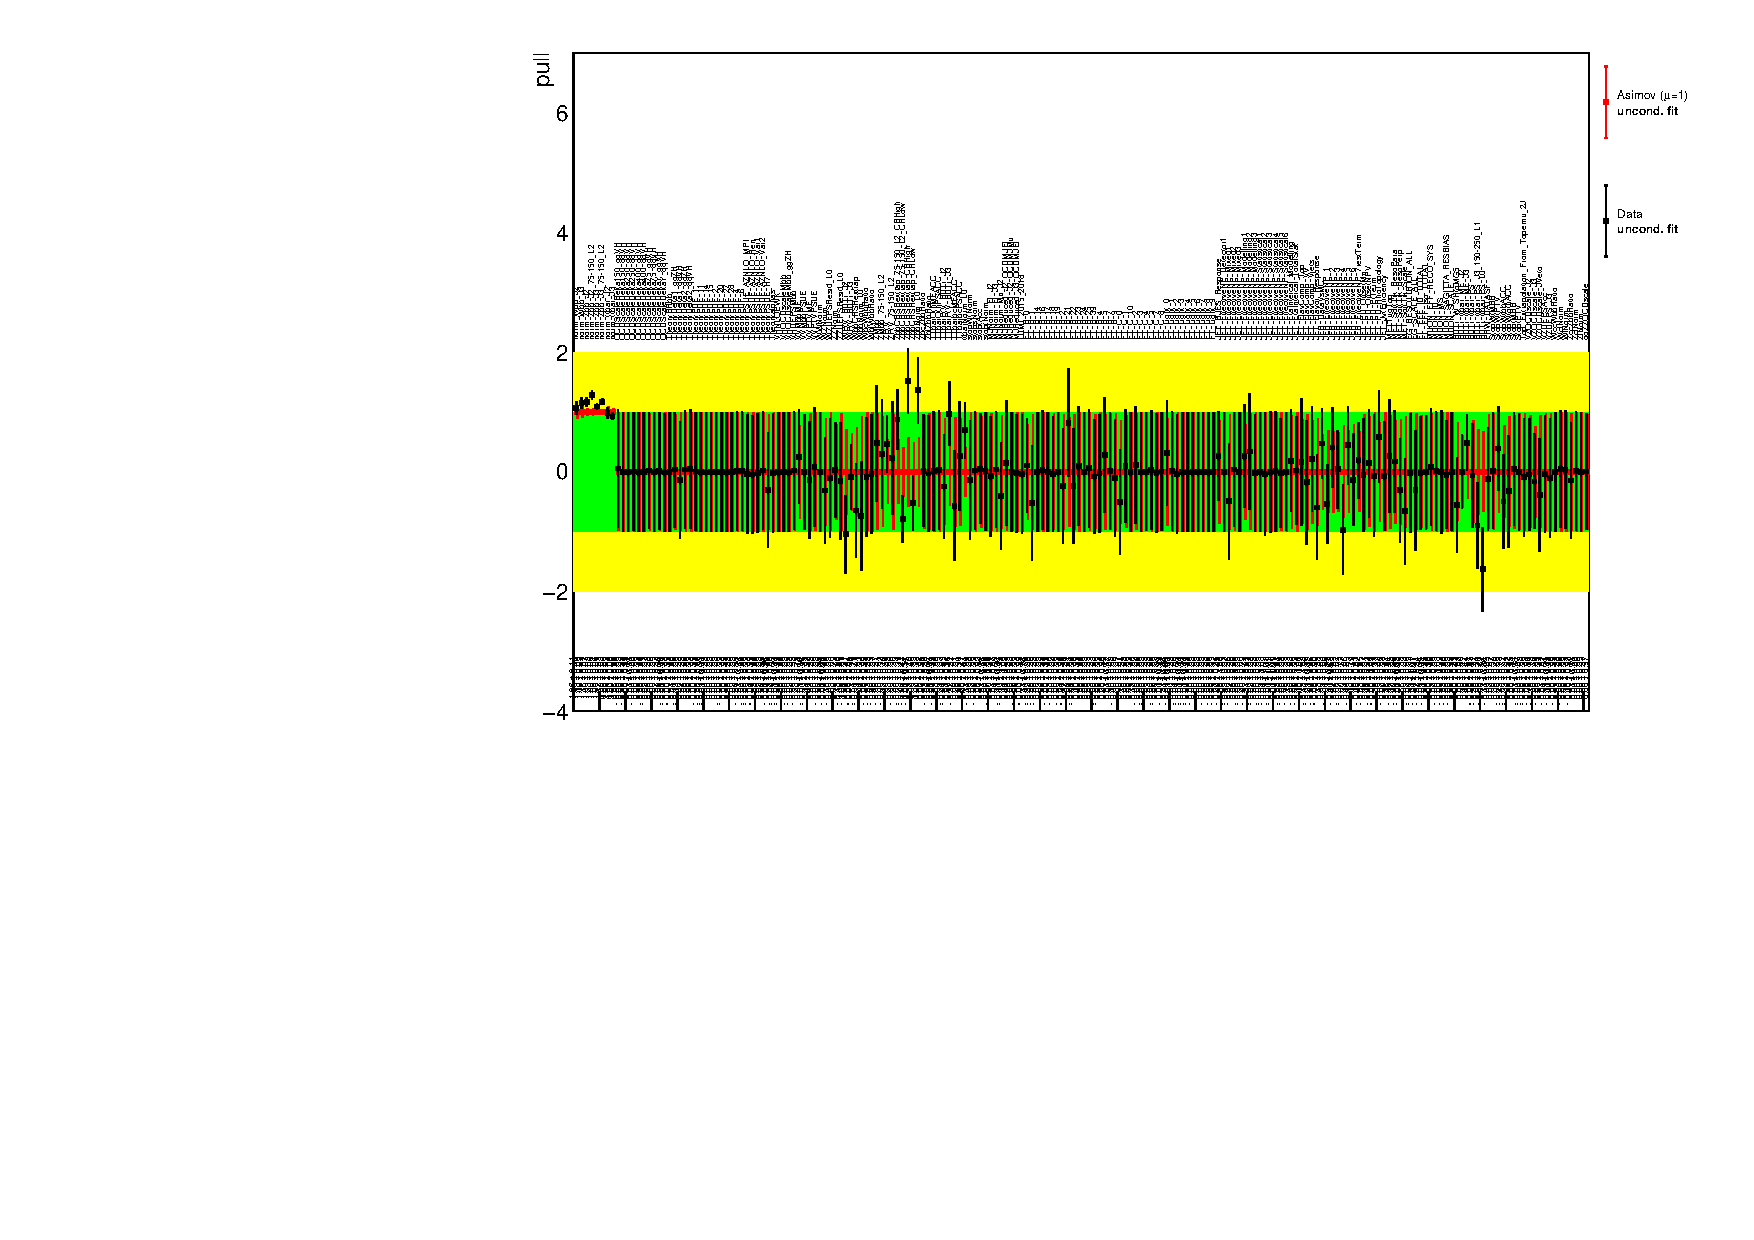
\includegraphics[angle=270]{final_fit_mva/pullComparisons/NP_allExceptGammas.pdf}
% \caption{caption}
% % Nuisance parameter pulls and the free parameter scale factors corresponding to
% % an unconditional combined fit performed to the Asimov dataset (red) and an
% % unconditional combined fit to the \RunTwo data (black).
% \label{fig:nppulls_012L_MVAVH} 
% \end{figure}
%
\begin{figure}[hb]
\centering
%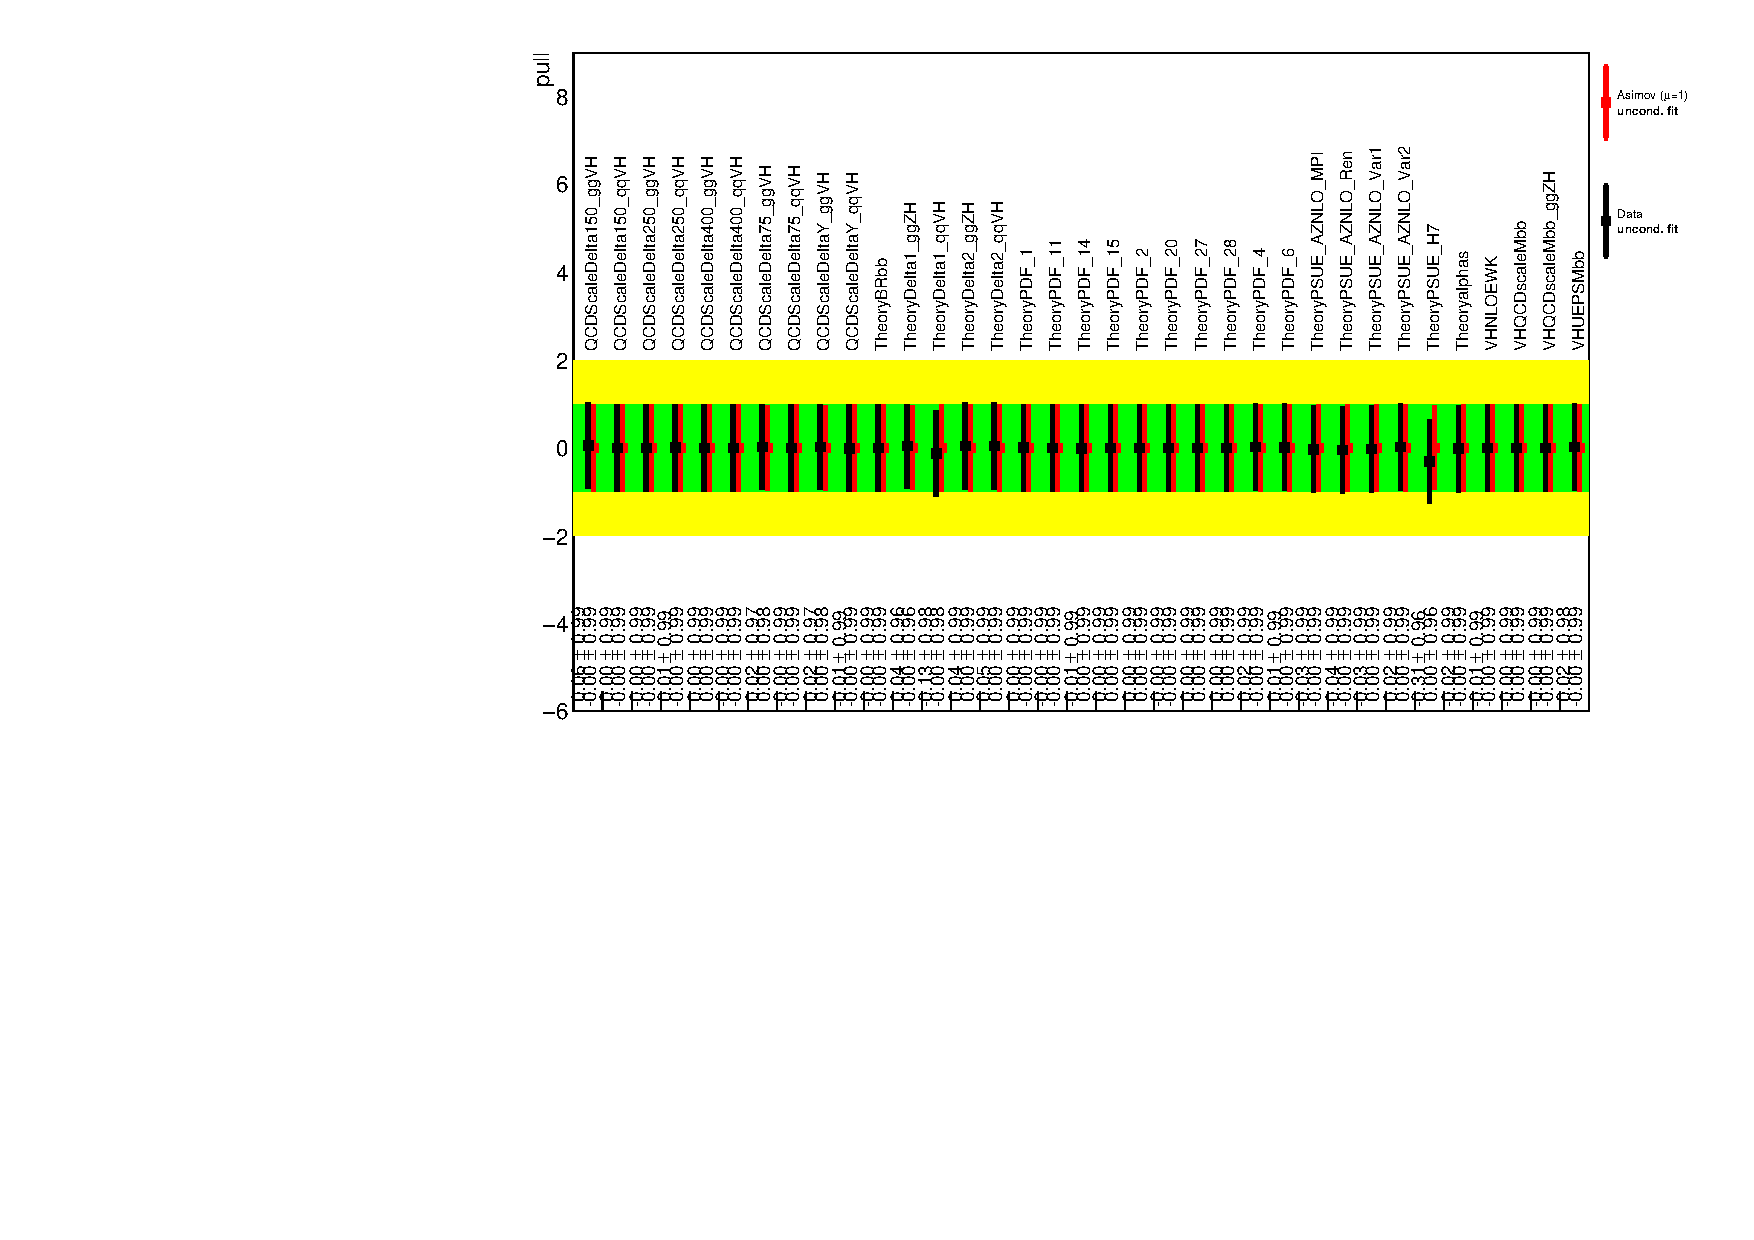
\includegraphics[width=0.49\linewidth]{final_fit_mva/pullComparisons/NP_VH.pdf}
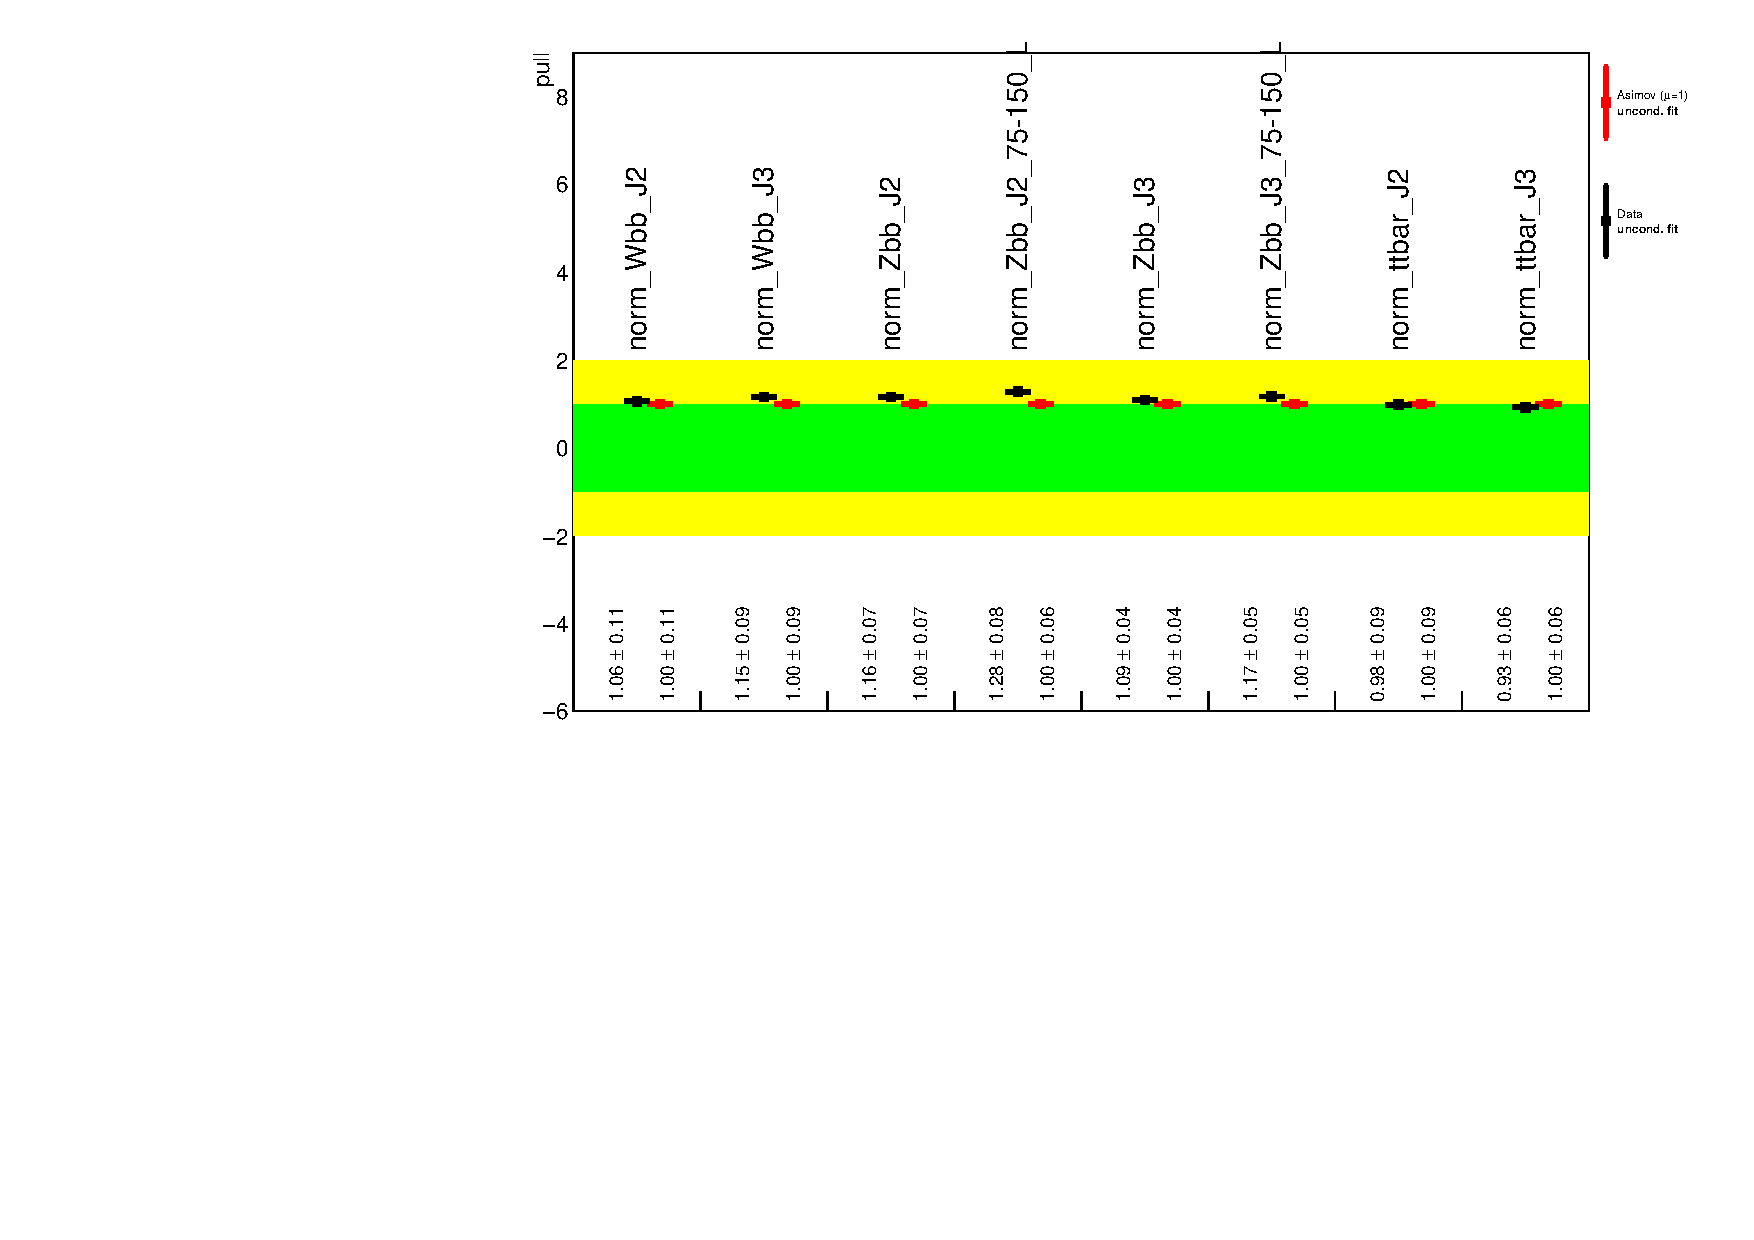
\includegraphics[width=0.49\linewidth]{final_fit_mva/pullComparisons/NP_FloatNorm.pdf}
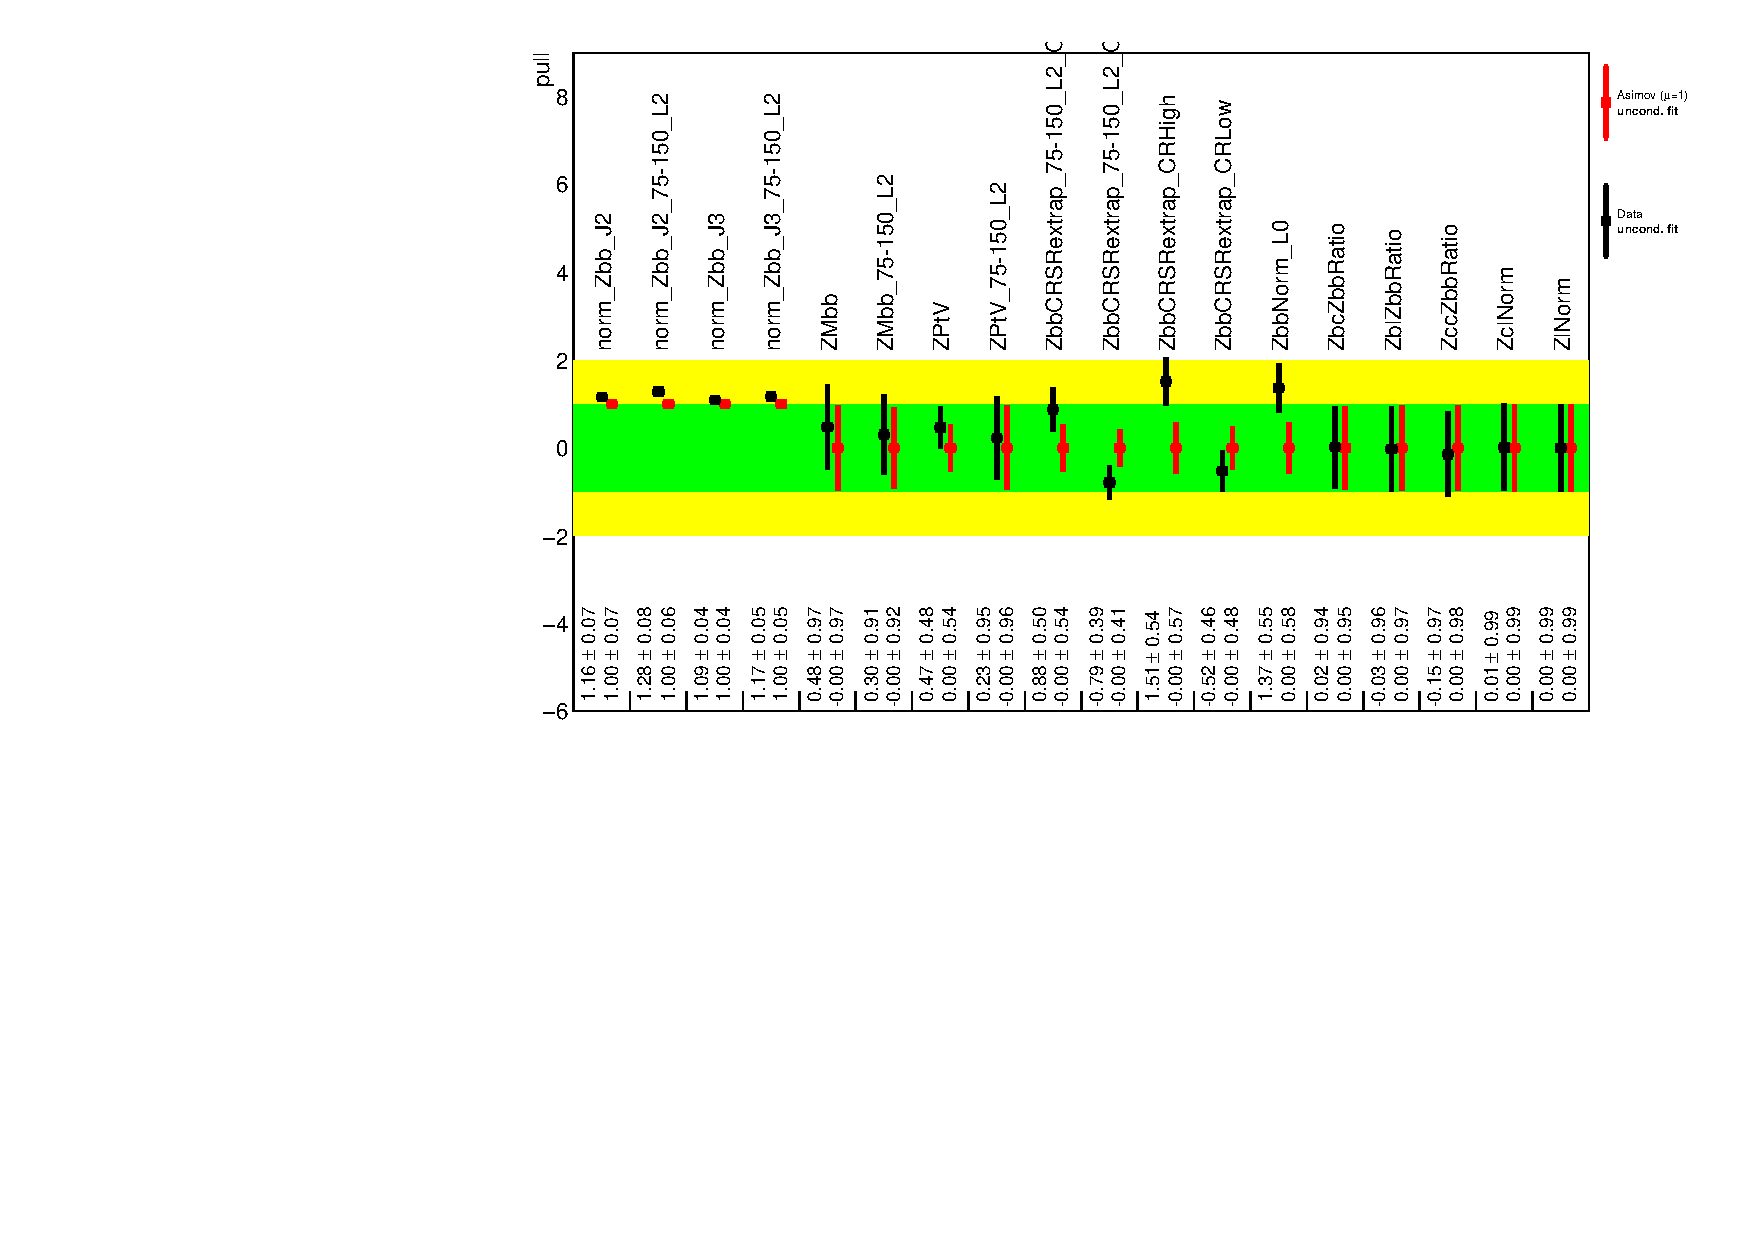
\includegraphics[width=0.49\linewidth]{final_fit_mva/pullComparisons/NP_Zjets.pdf}
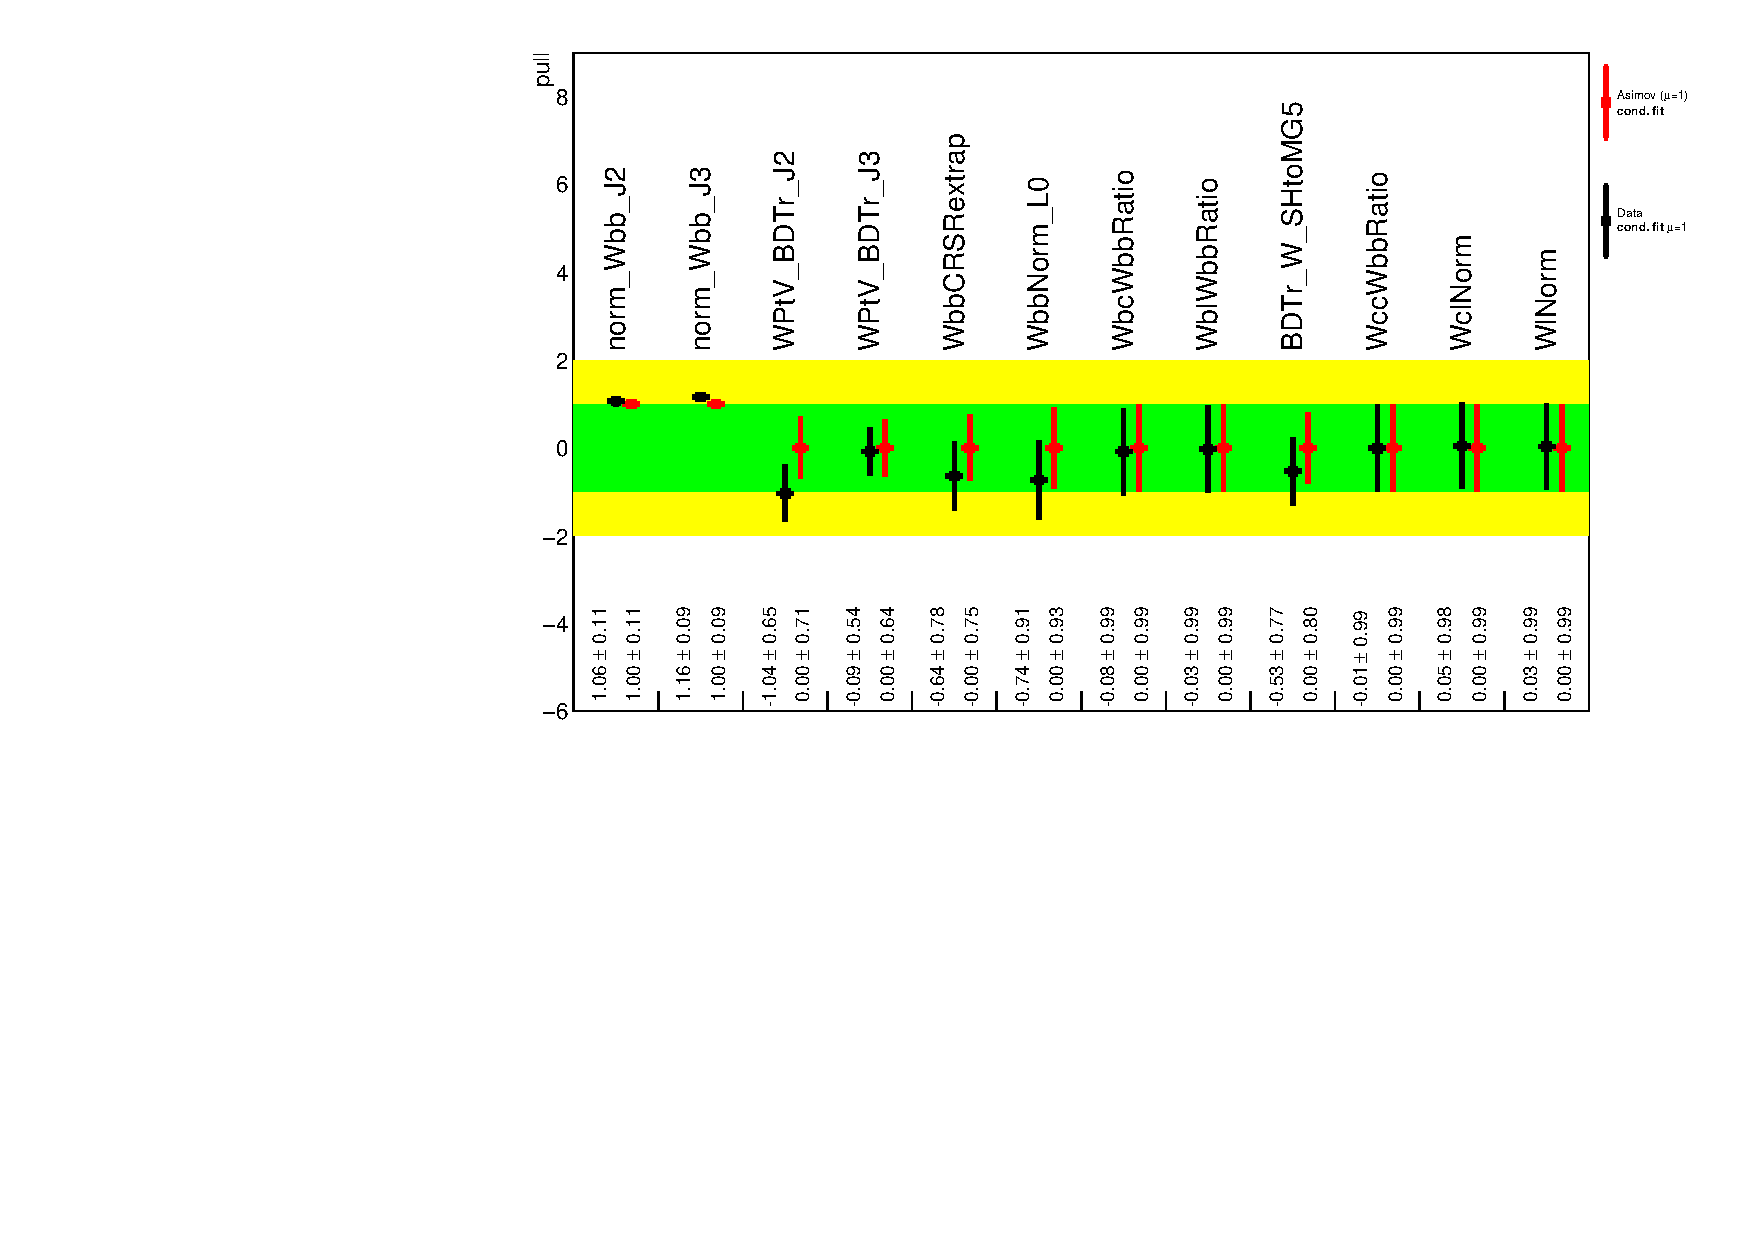
\includegraphics[width=0.49\linewidth]{final_fit_mva/pullComparisons/NP_Wjets.pdf}
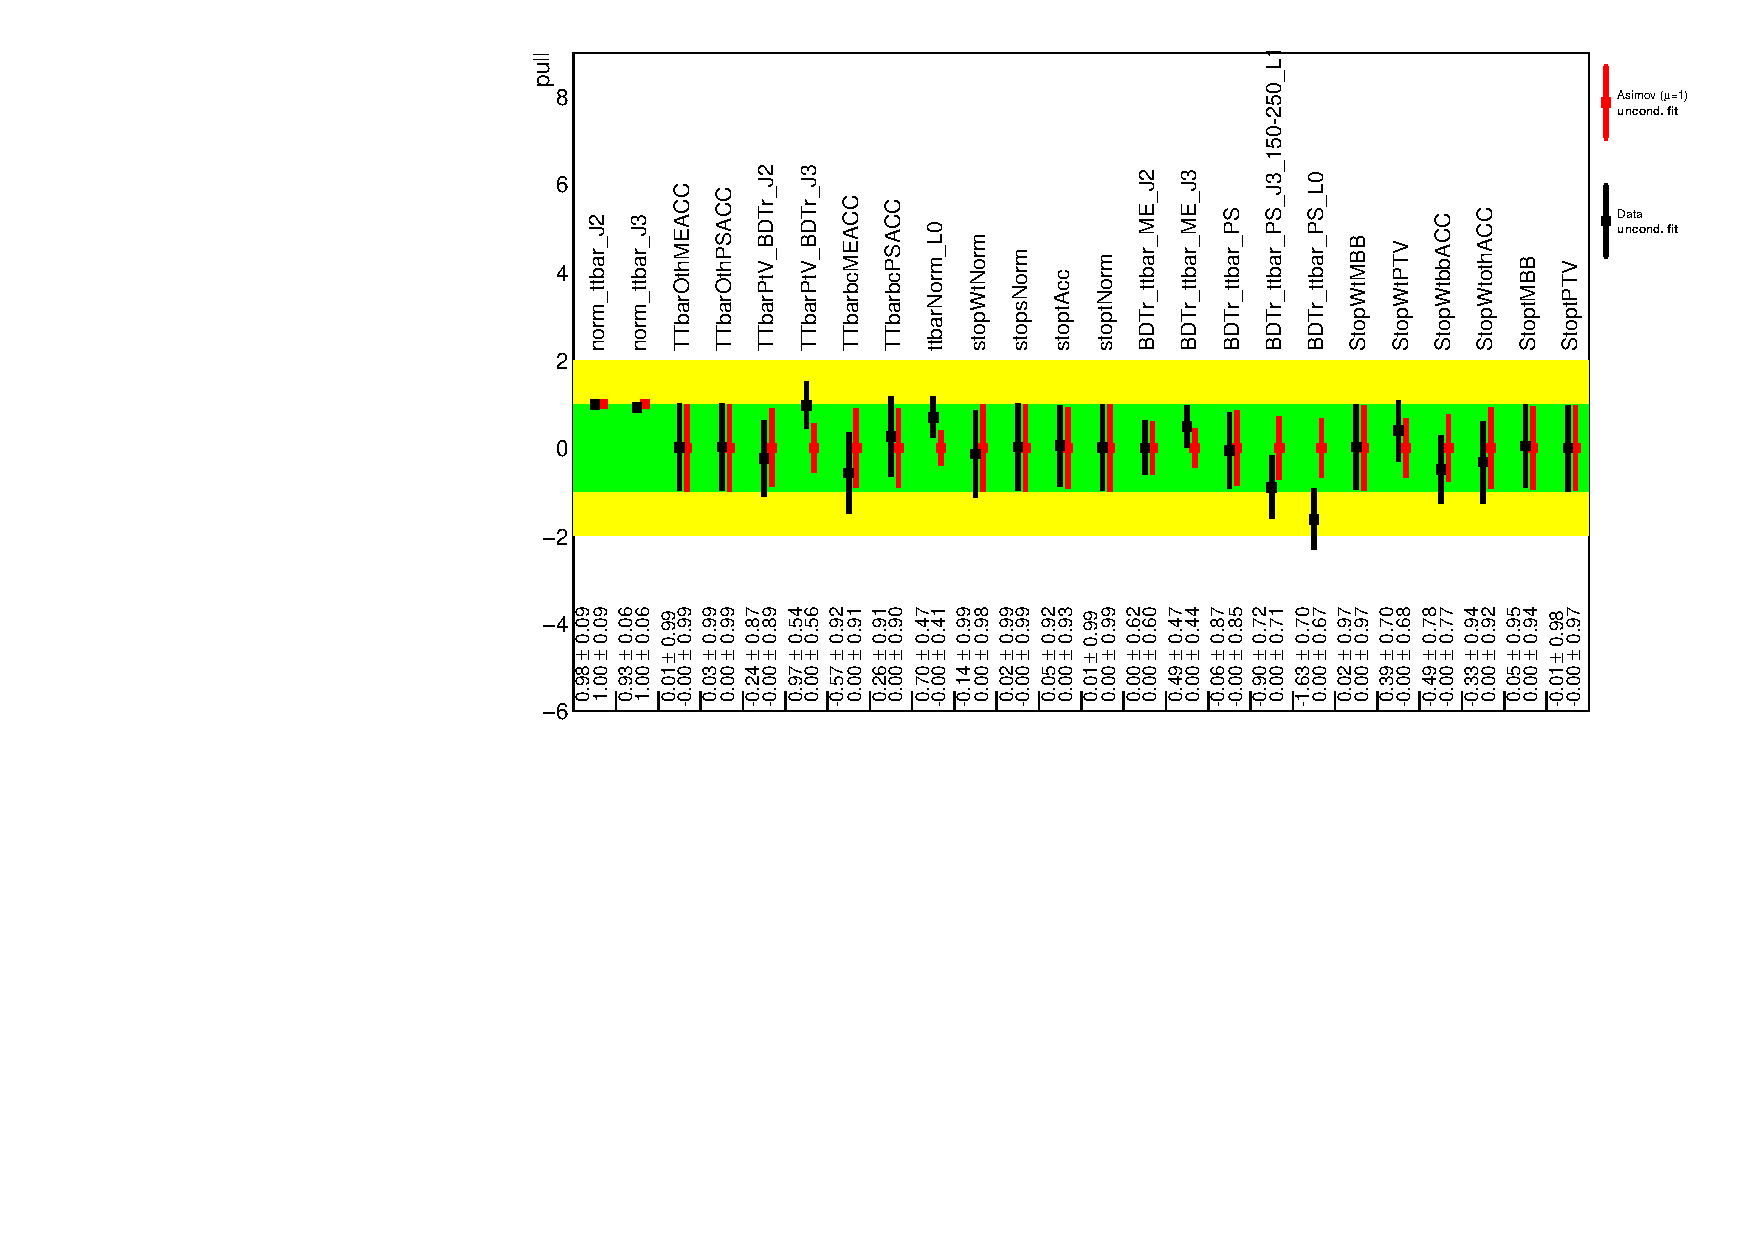
\includegraphics[width=0.49\linewidth]{final_fit_mva/pullComparisons/NP_Top.pdf}
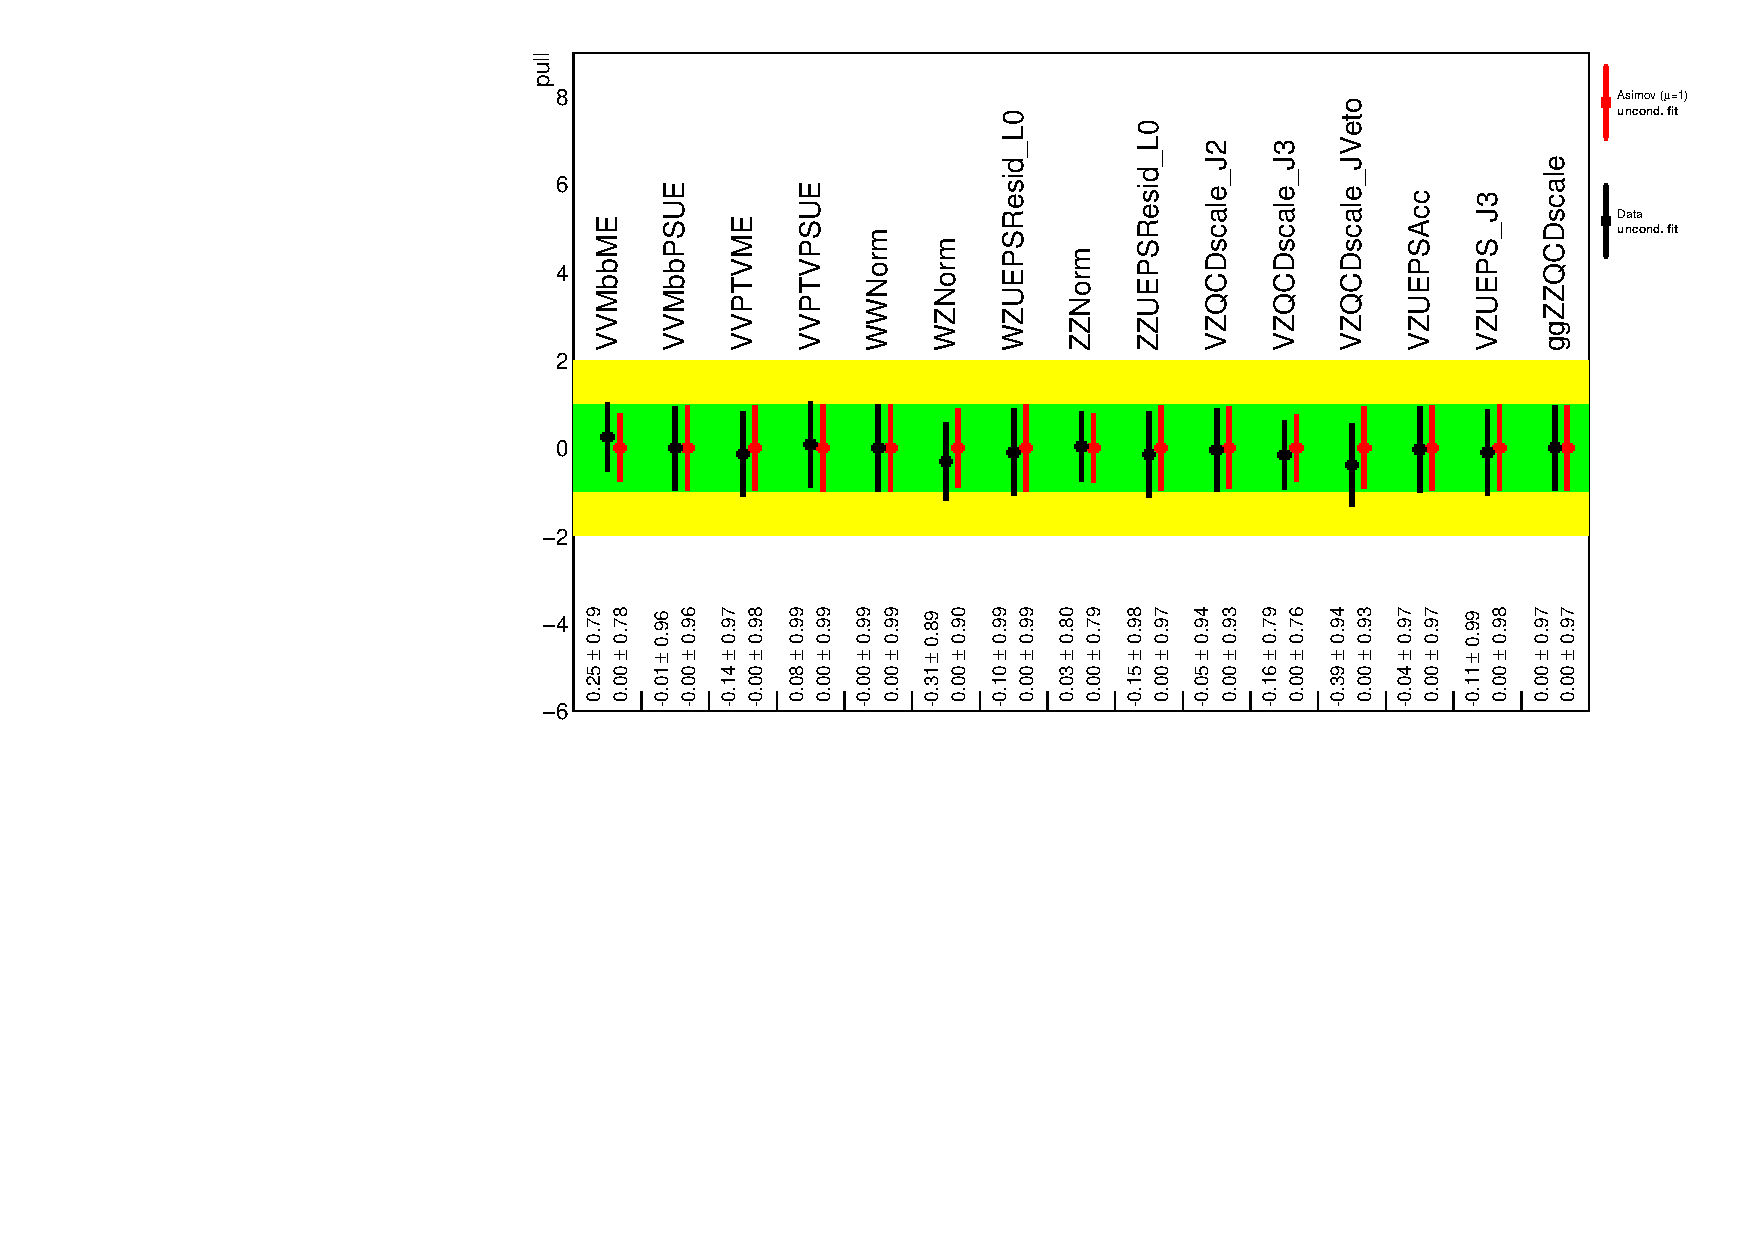
\includegraphics[width=0.49\linewidth]{final_fit_mva/pullComparisons/NP_Diboson.pdf}
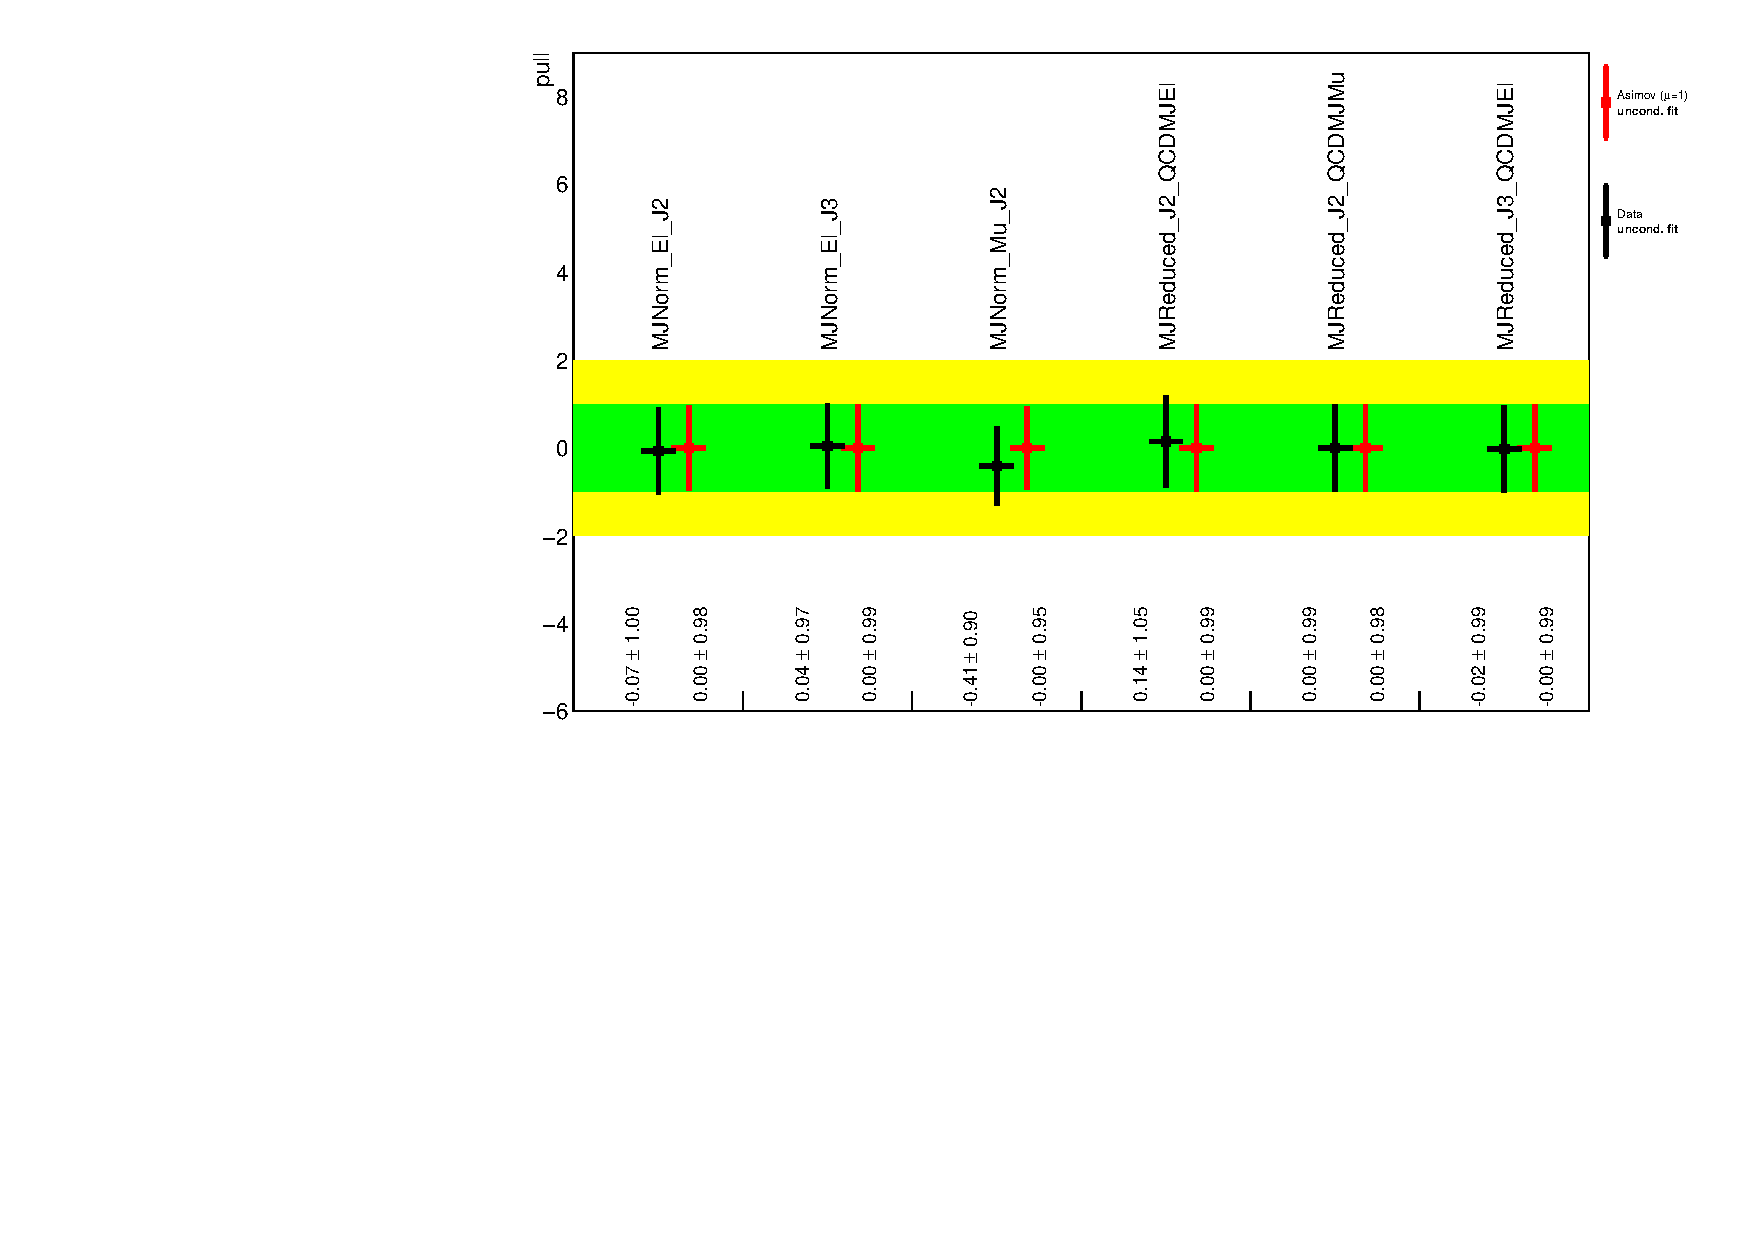
\includegraphics[width=0.49\linewidth]{final_fit_mva/pullComparisons/NP_MJ.pdf}
\caption{Nuisance parameter pulls and free parameter scale factors relating
  to the backgrounds of the analysis, where an Asimov dataset conditional on
  $\mu=1$ in red is compared with the data in black.}
\label{fig:nppulls_012L_MVAVH_a} 
\end{figure}
%
\begin{figure}[hb]
\centering
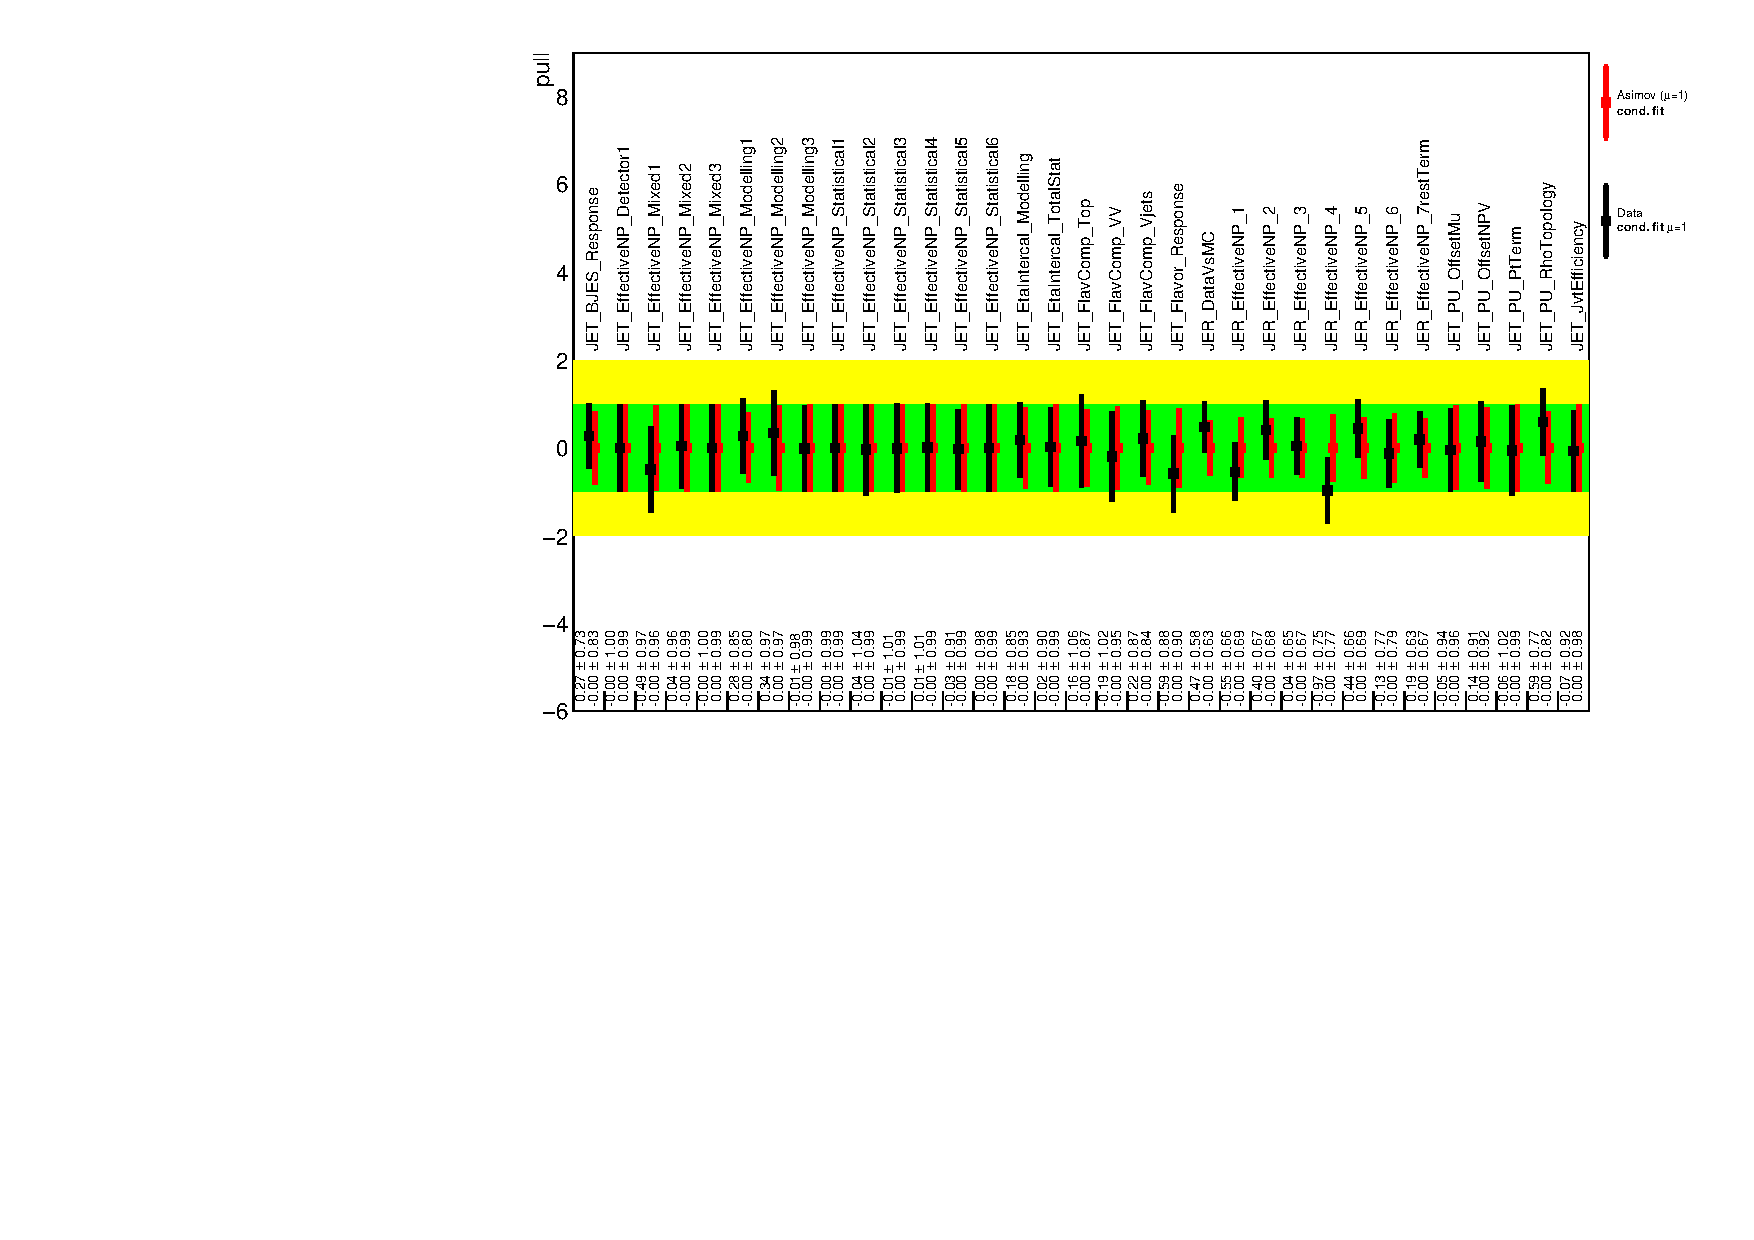
\includegraphics[width=0.49\linewidth]{final_fit_mva/pullComparisons/NP_Jet.pdf}
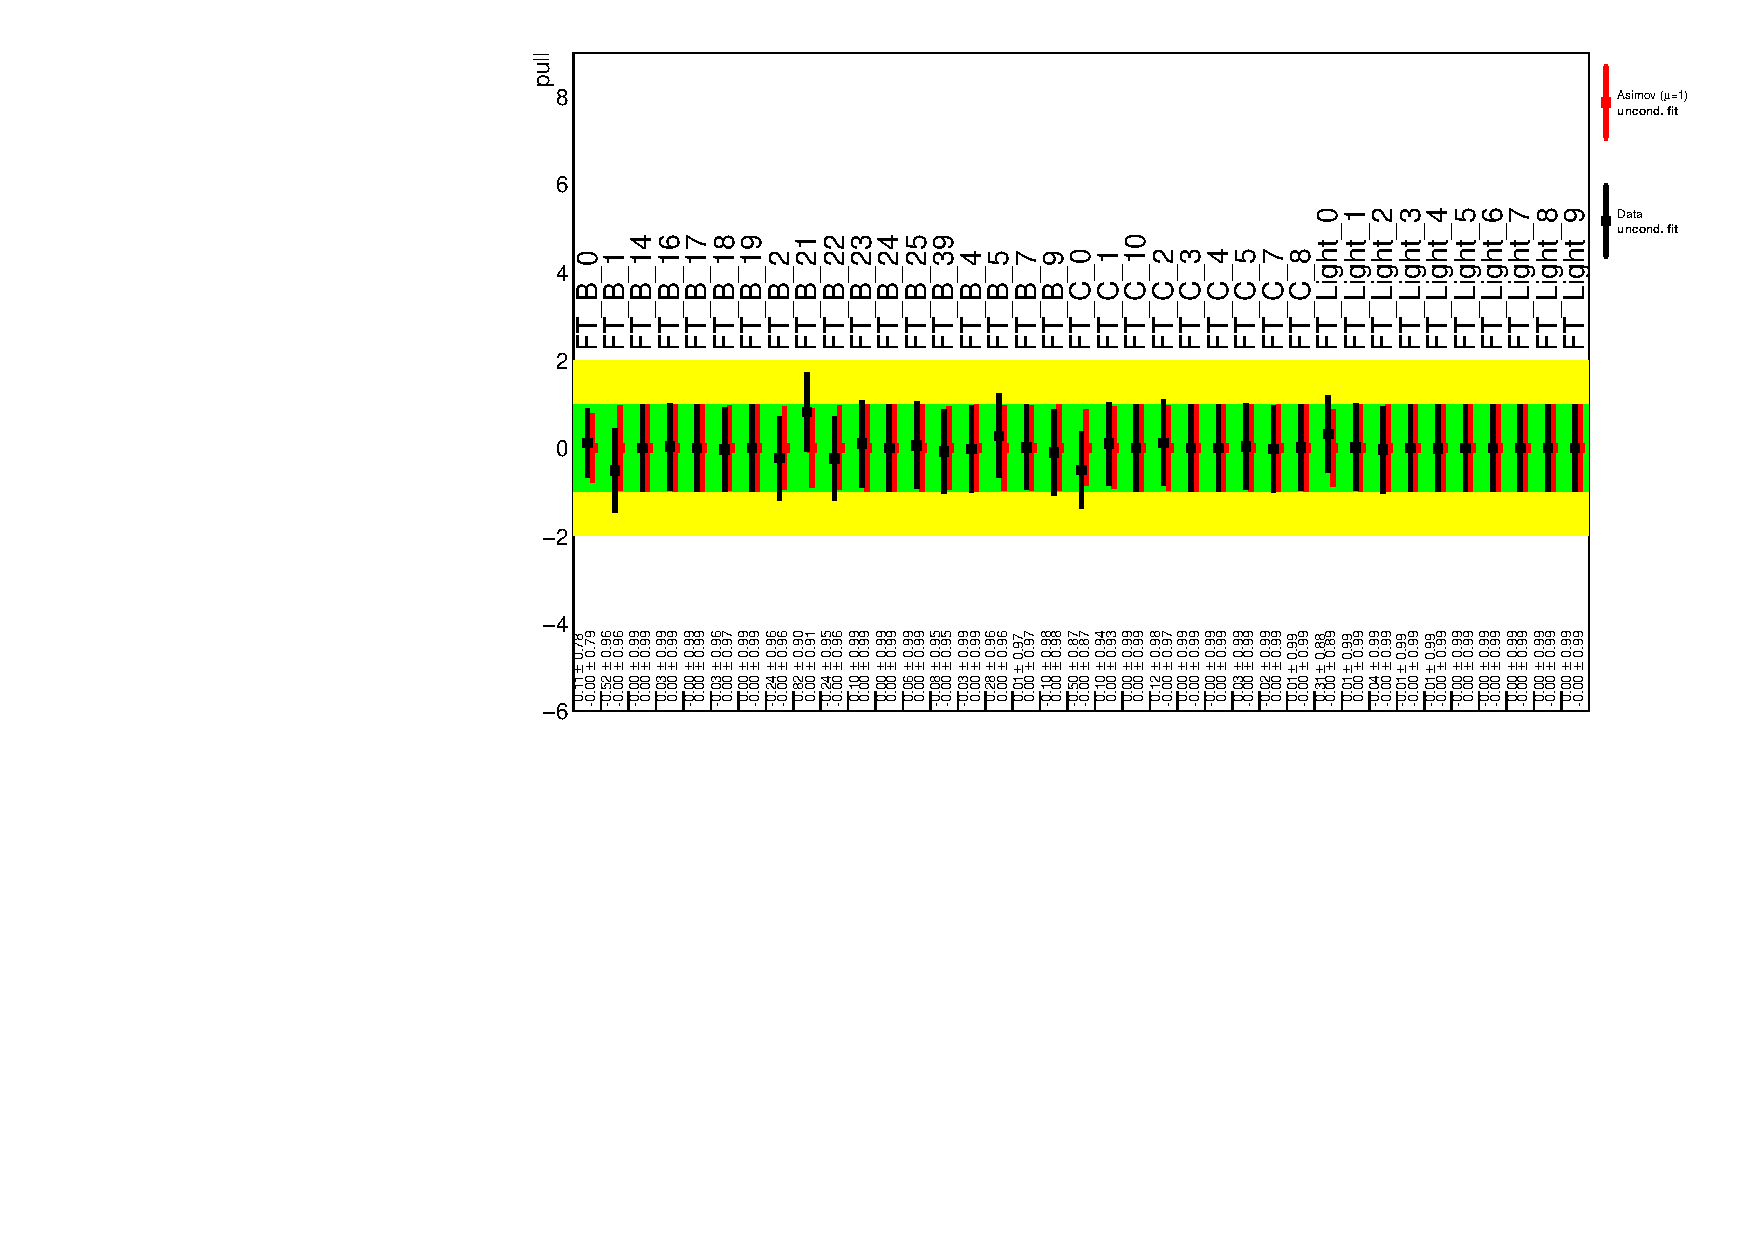
\includegraphics[width=0.49\linewidth]{final_fit_mva/pullComparisons/NP_BTag.pdf}
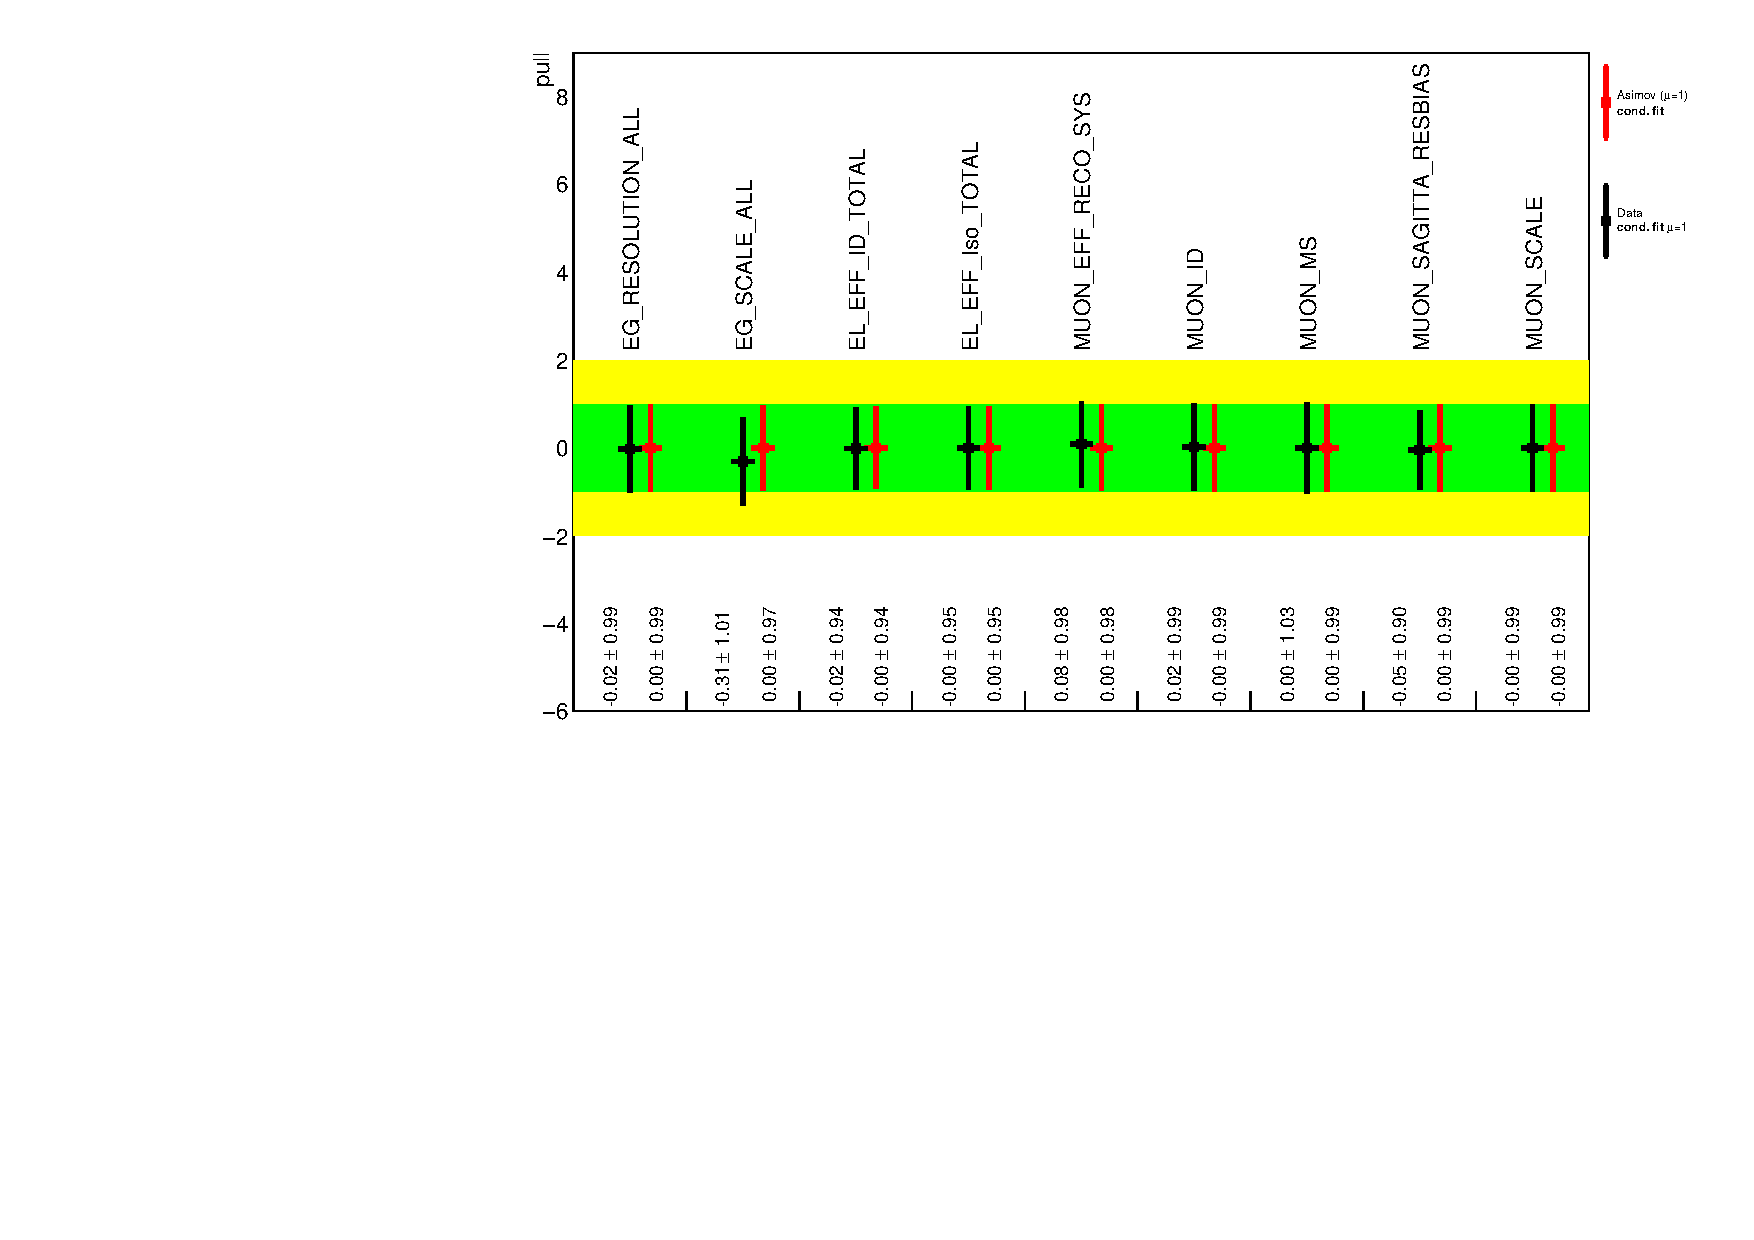
\includegraphics[width=0.49\linewidth]{final_fit_mva/pullComparisons/NP_Lepton.pdf}
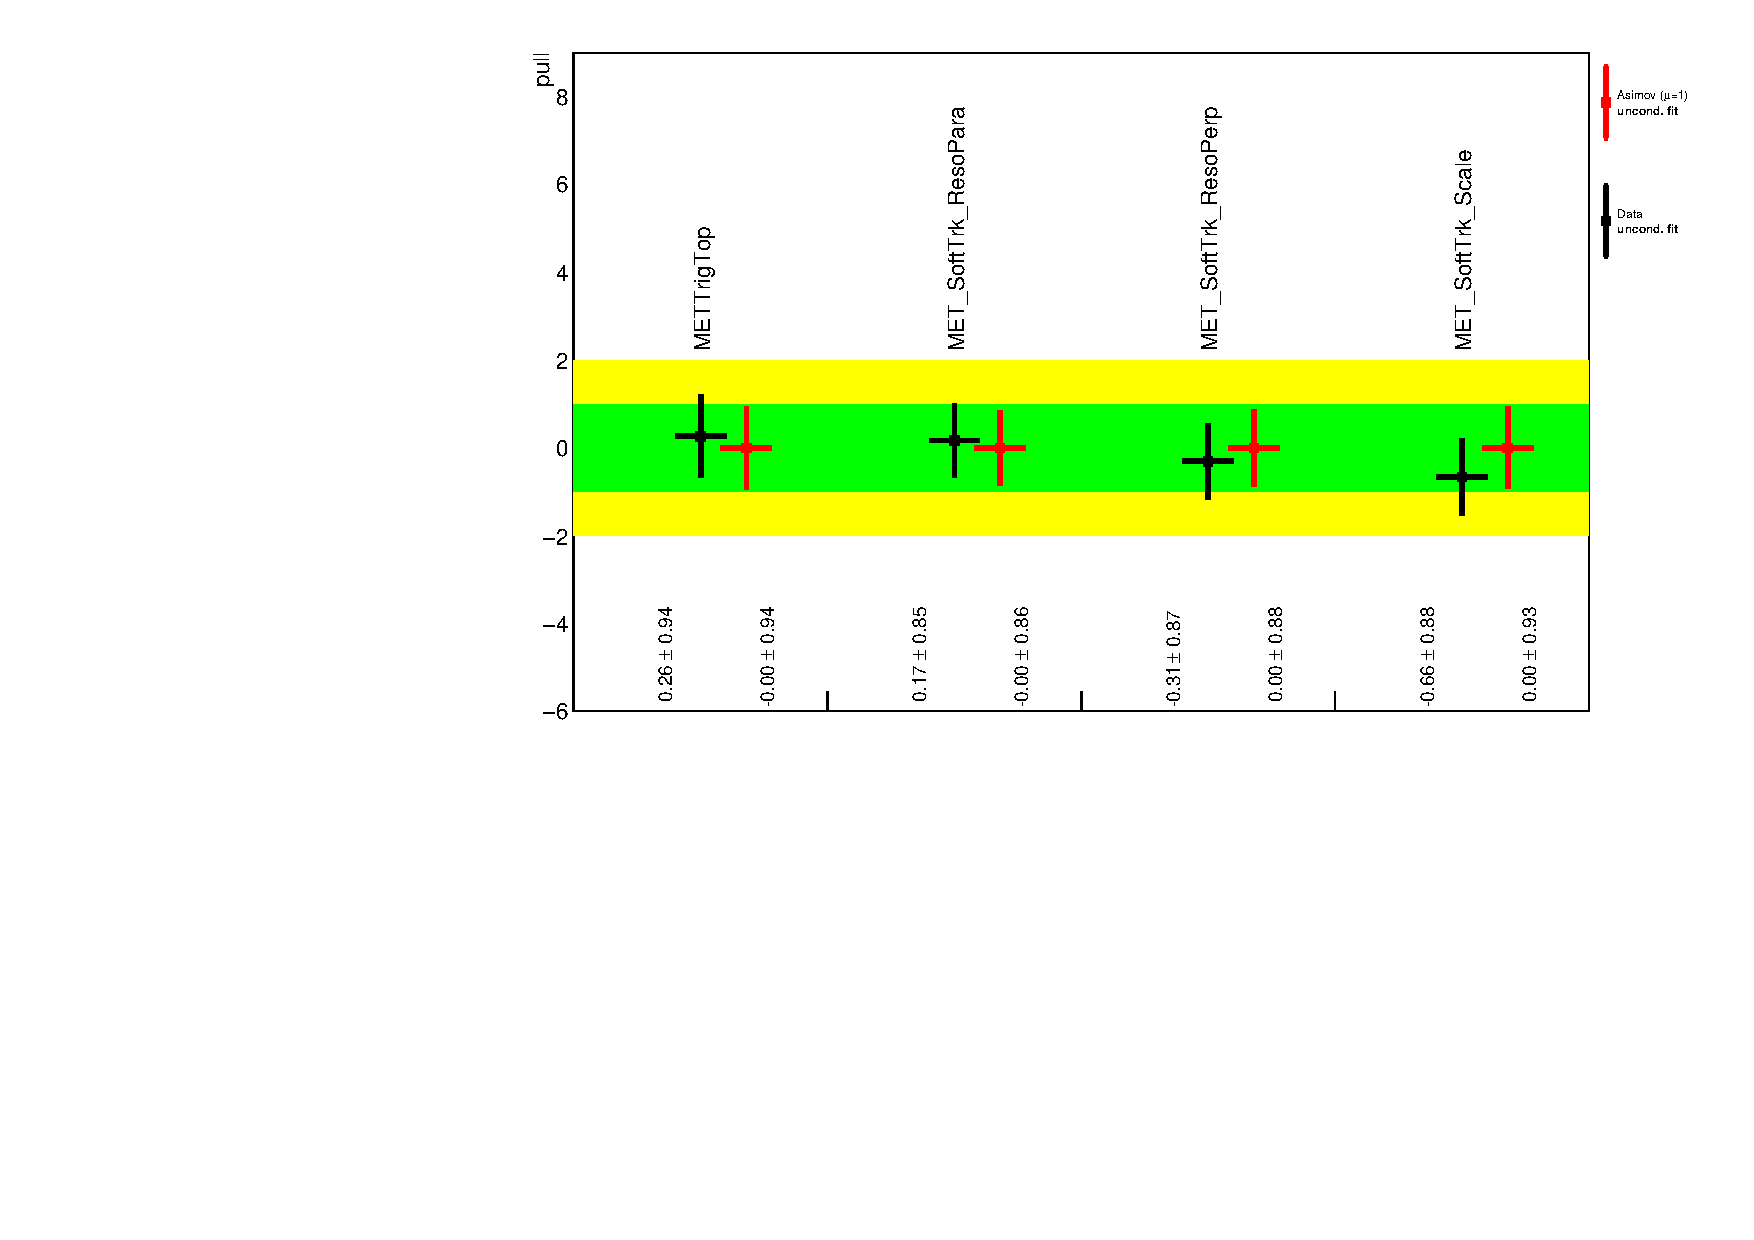
\includegraphics[width=0.49\linewidth]{final_fit_mva/pullComparisons/NP_MET.pdf}
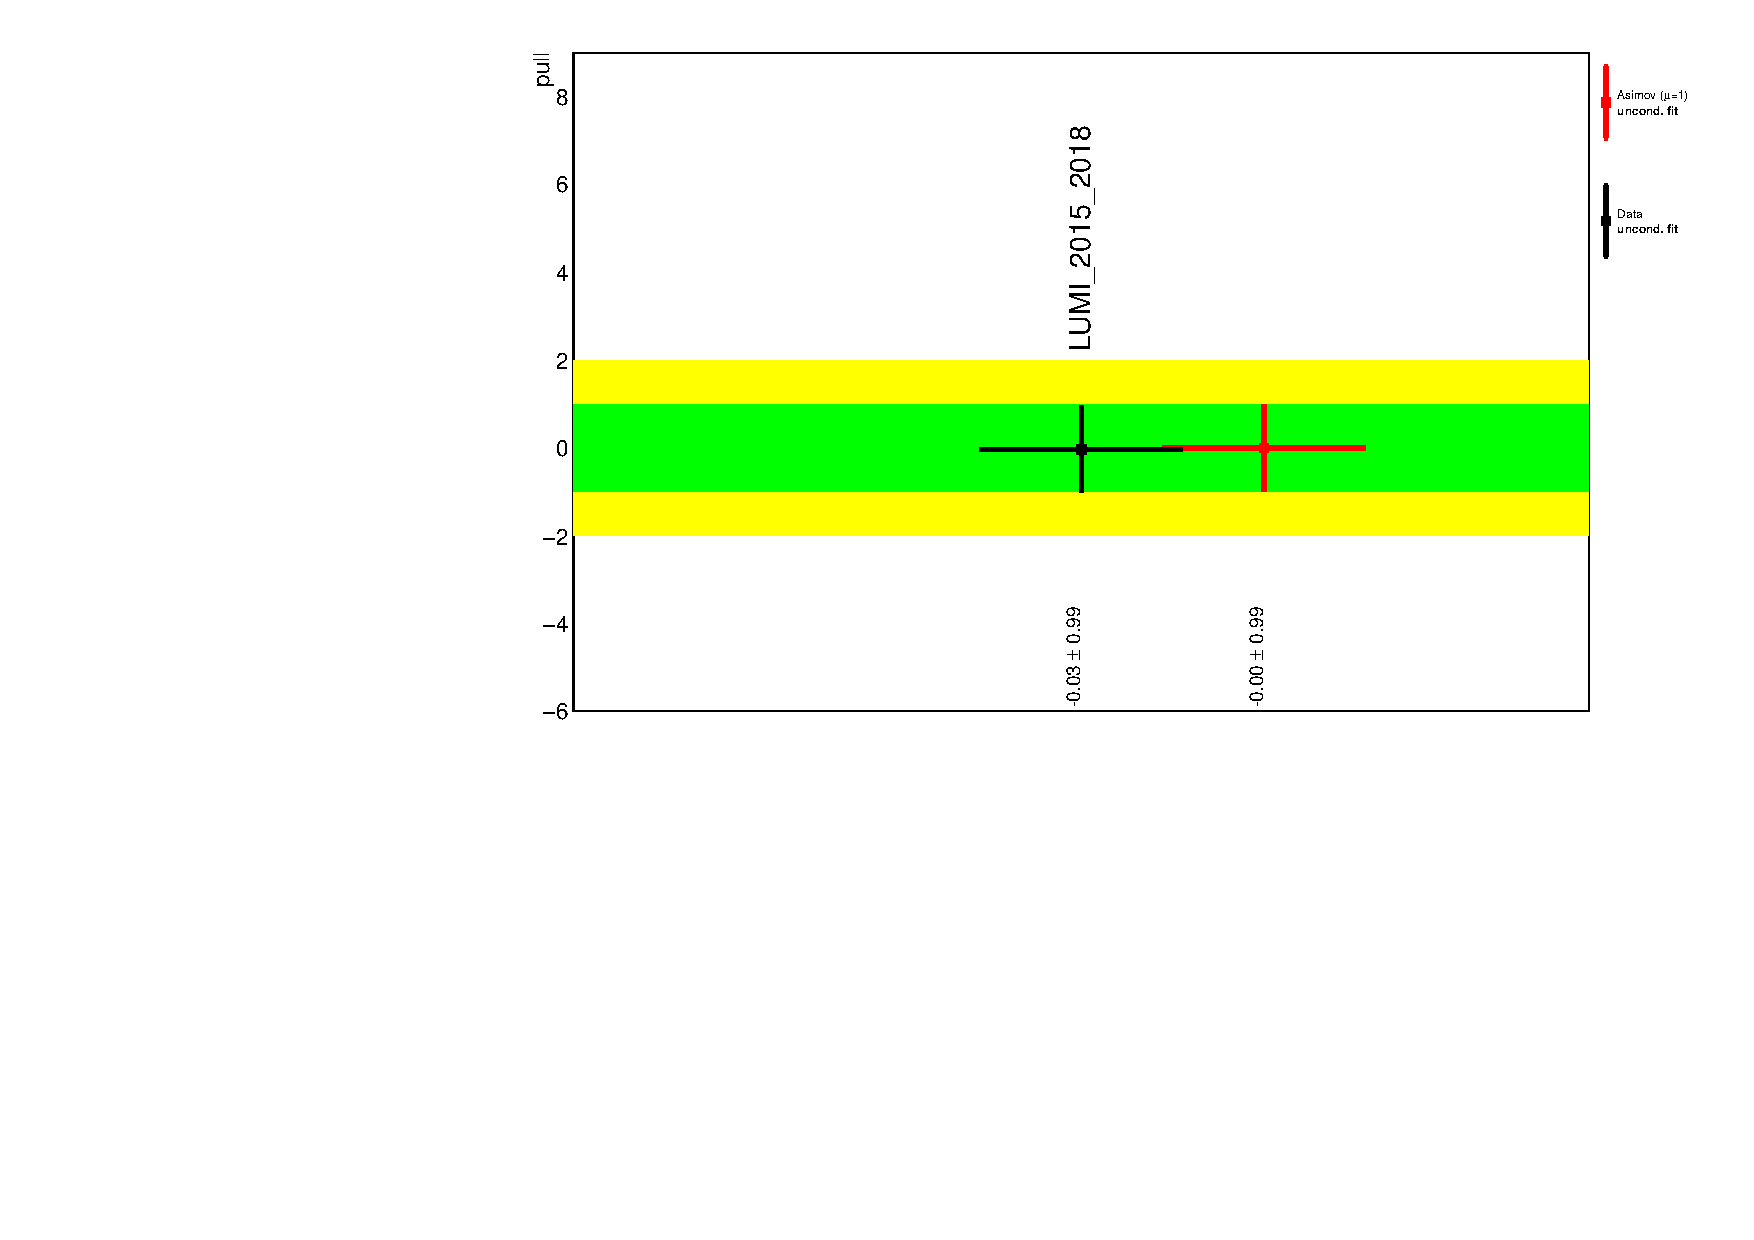
\includegraphics[width=0.49\linewidth]{final_fit_mva/pullComparisons/NP_LUMI.pdf}
\caption{Nuisance parameter pulls and free parameter scale factors relating to the
  experimental sources of uncertainty in the the analysis, where an Asimov
  dataset conditional on $\mu=1$ in red is compared with the data in black.}
\label{fig:nppulls_012L_MVAVH_b}
\end{figure}
%
% \begin{figure}[hb]
% \centering
% 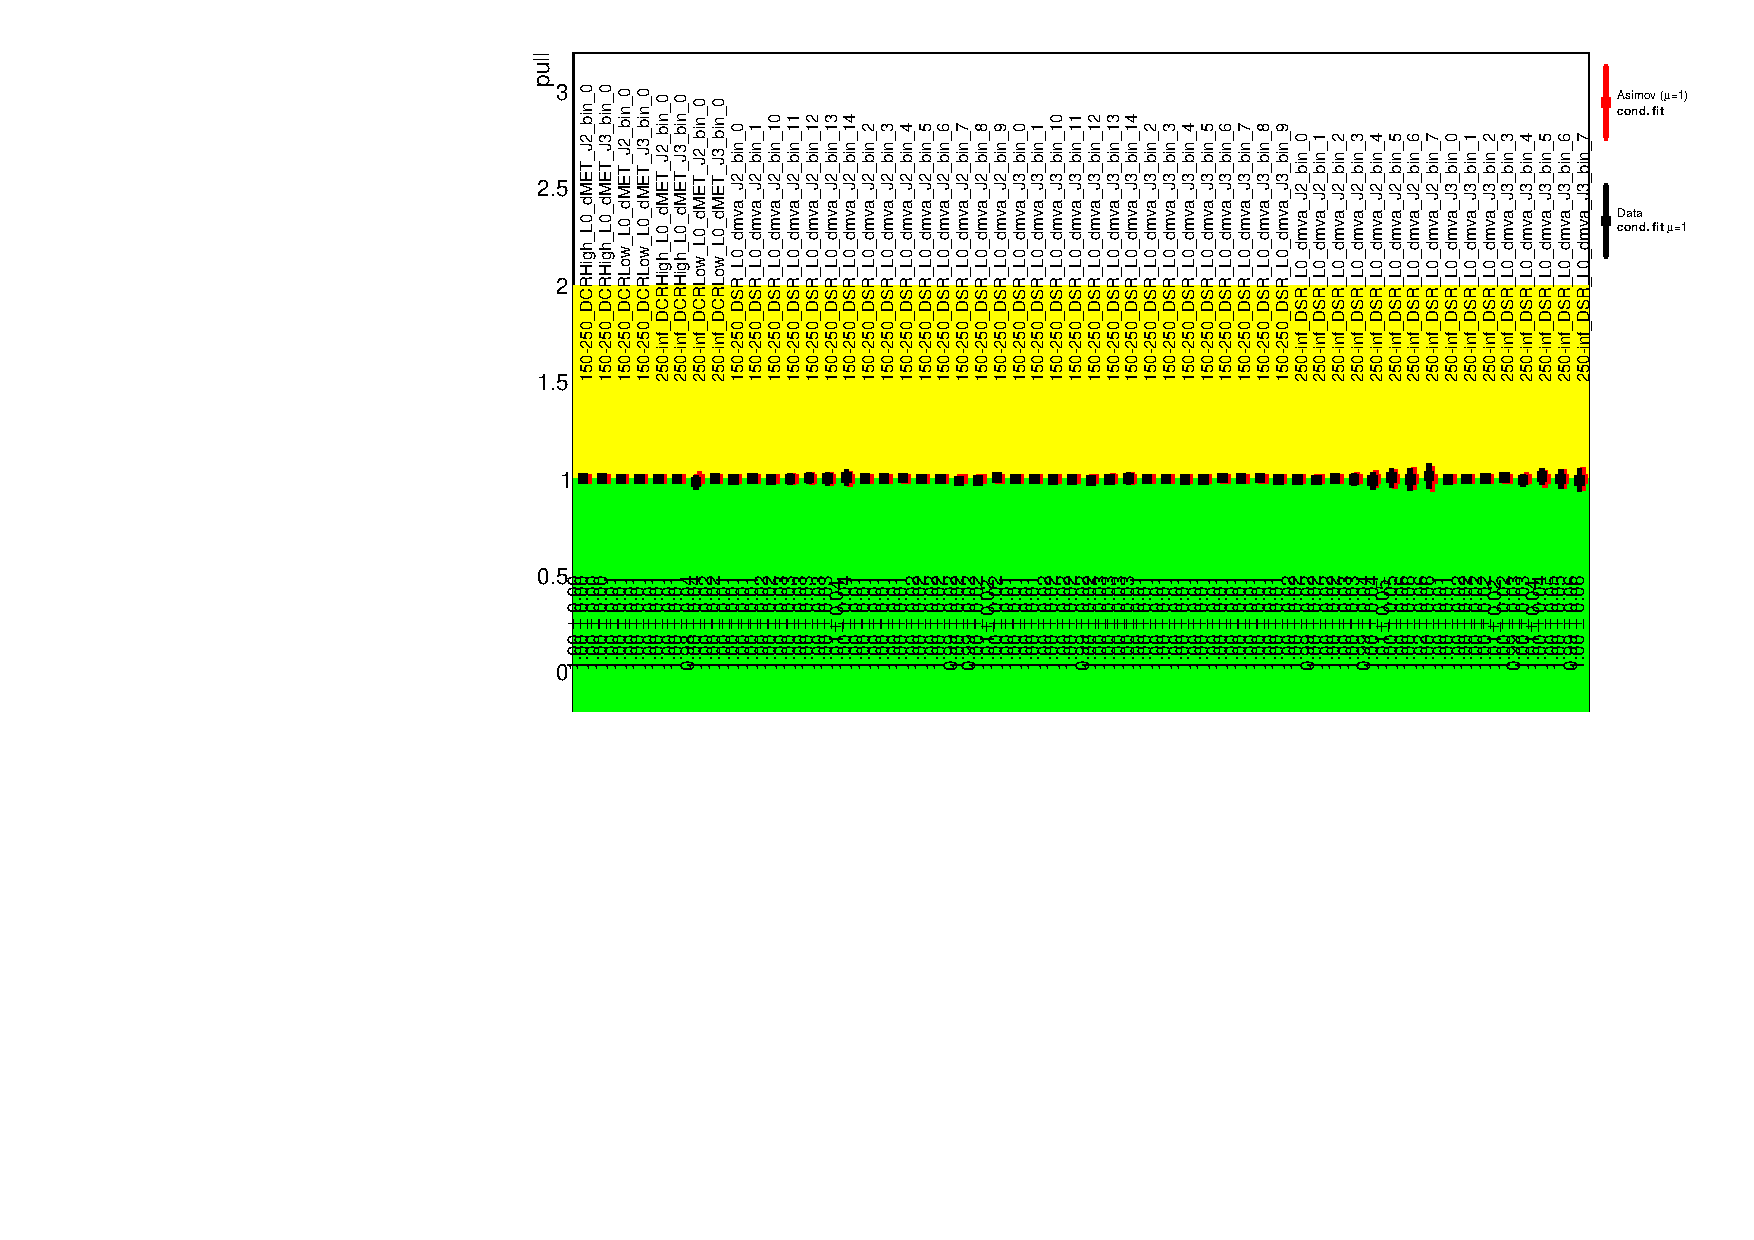
\includegraphics[width=0.49\linewidth]{final_fit_mva/pullComparisons/NP_GammasL0.pdf}
% 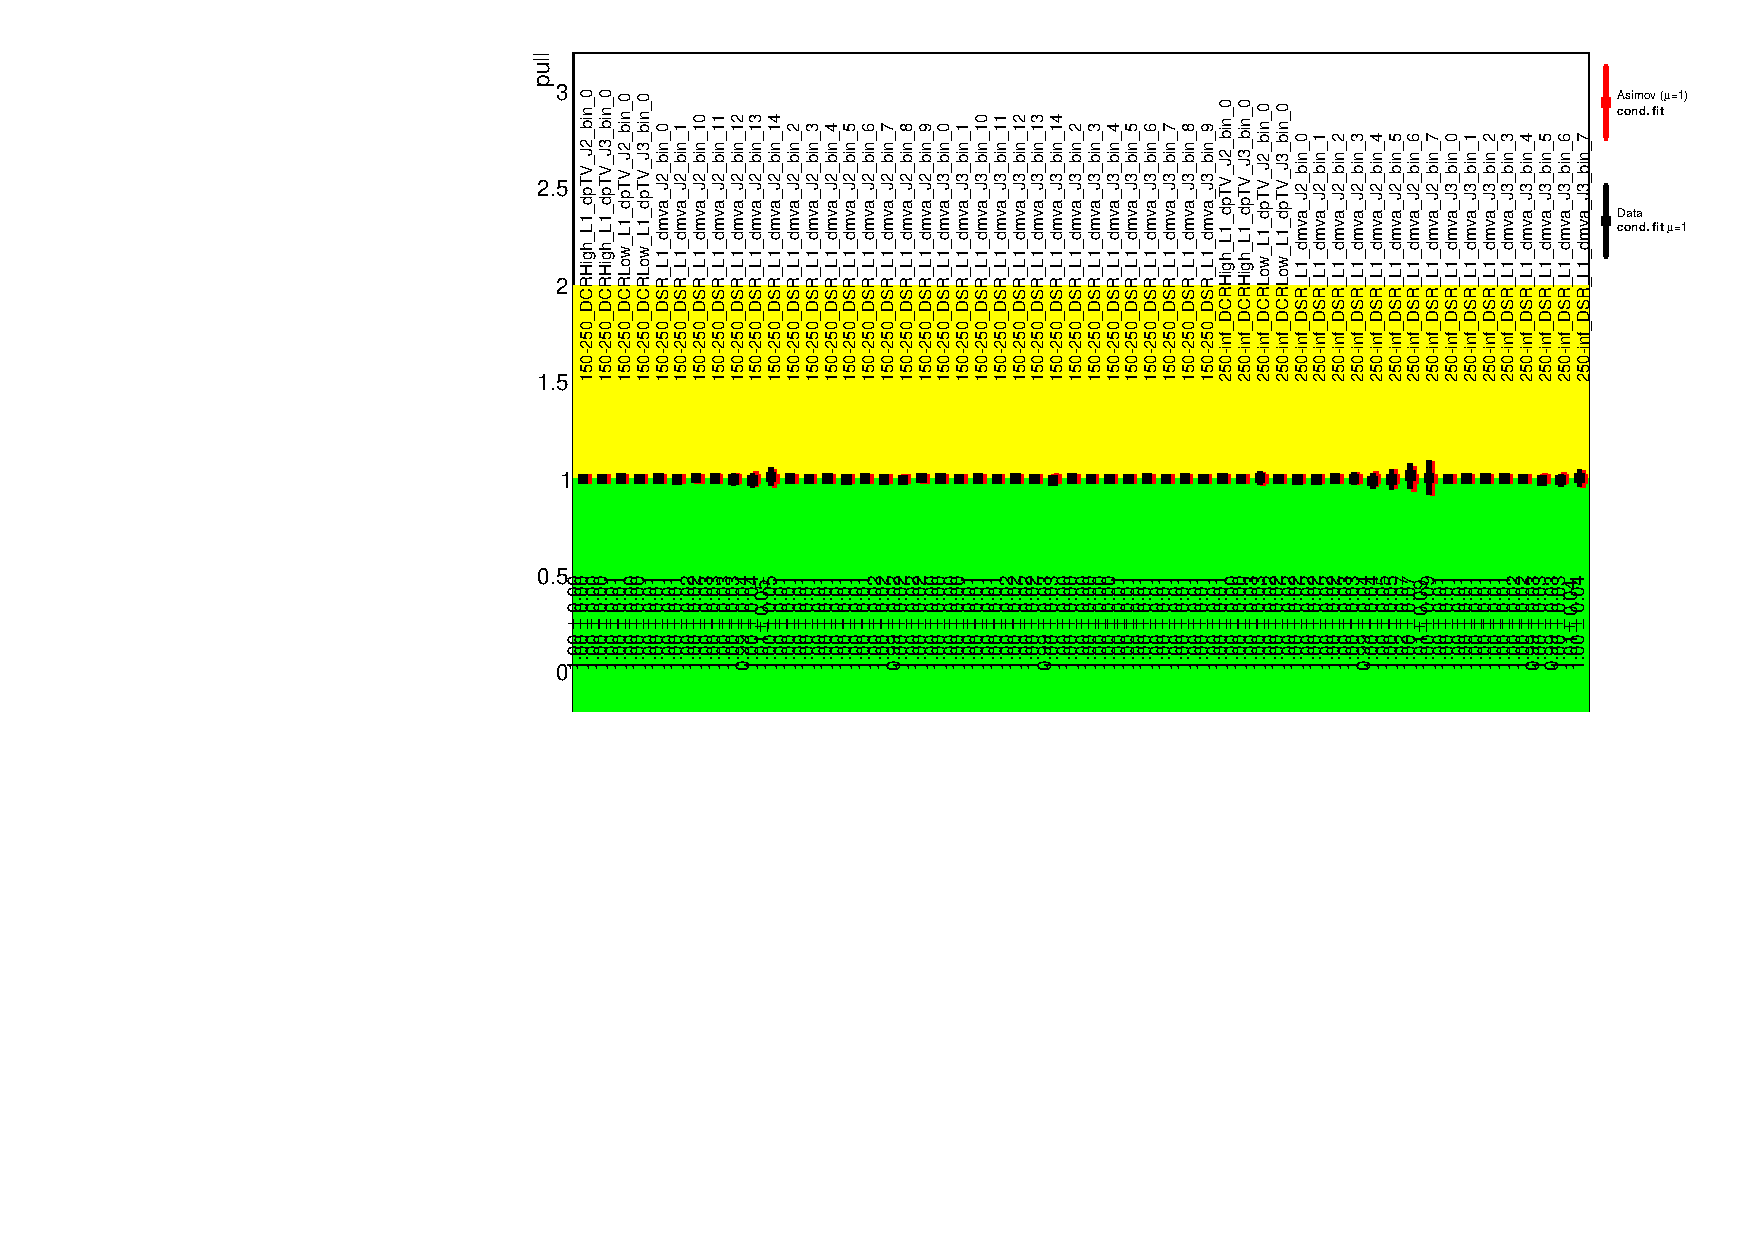
\includegraphics[width=0.49\linewidth]{final_fit_mva/pullComparisons/NP_GammasL1.pdf}
% 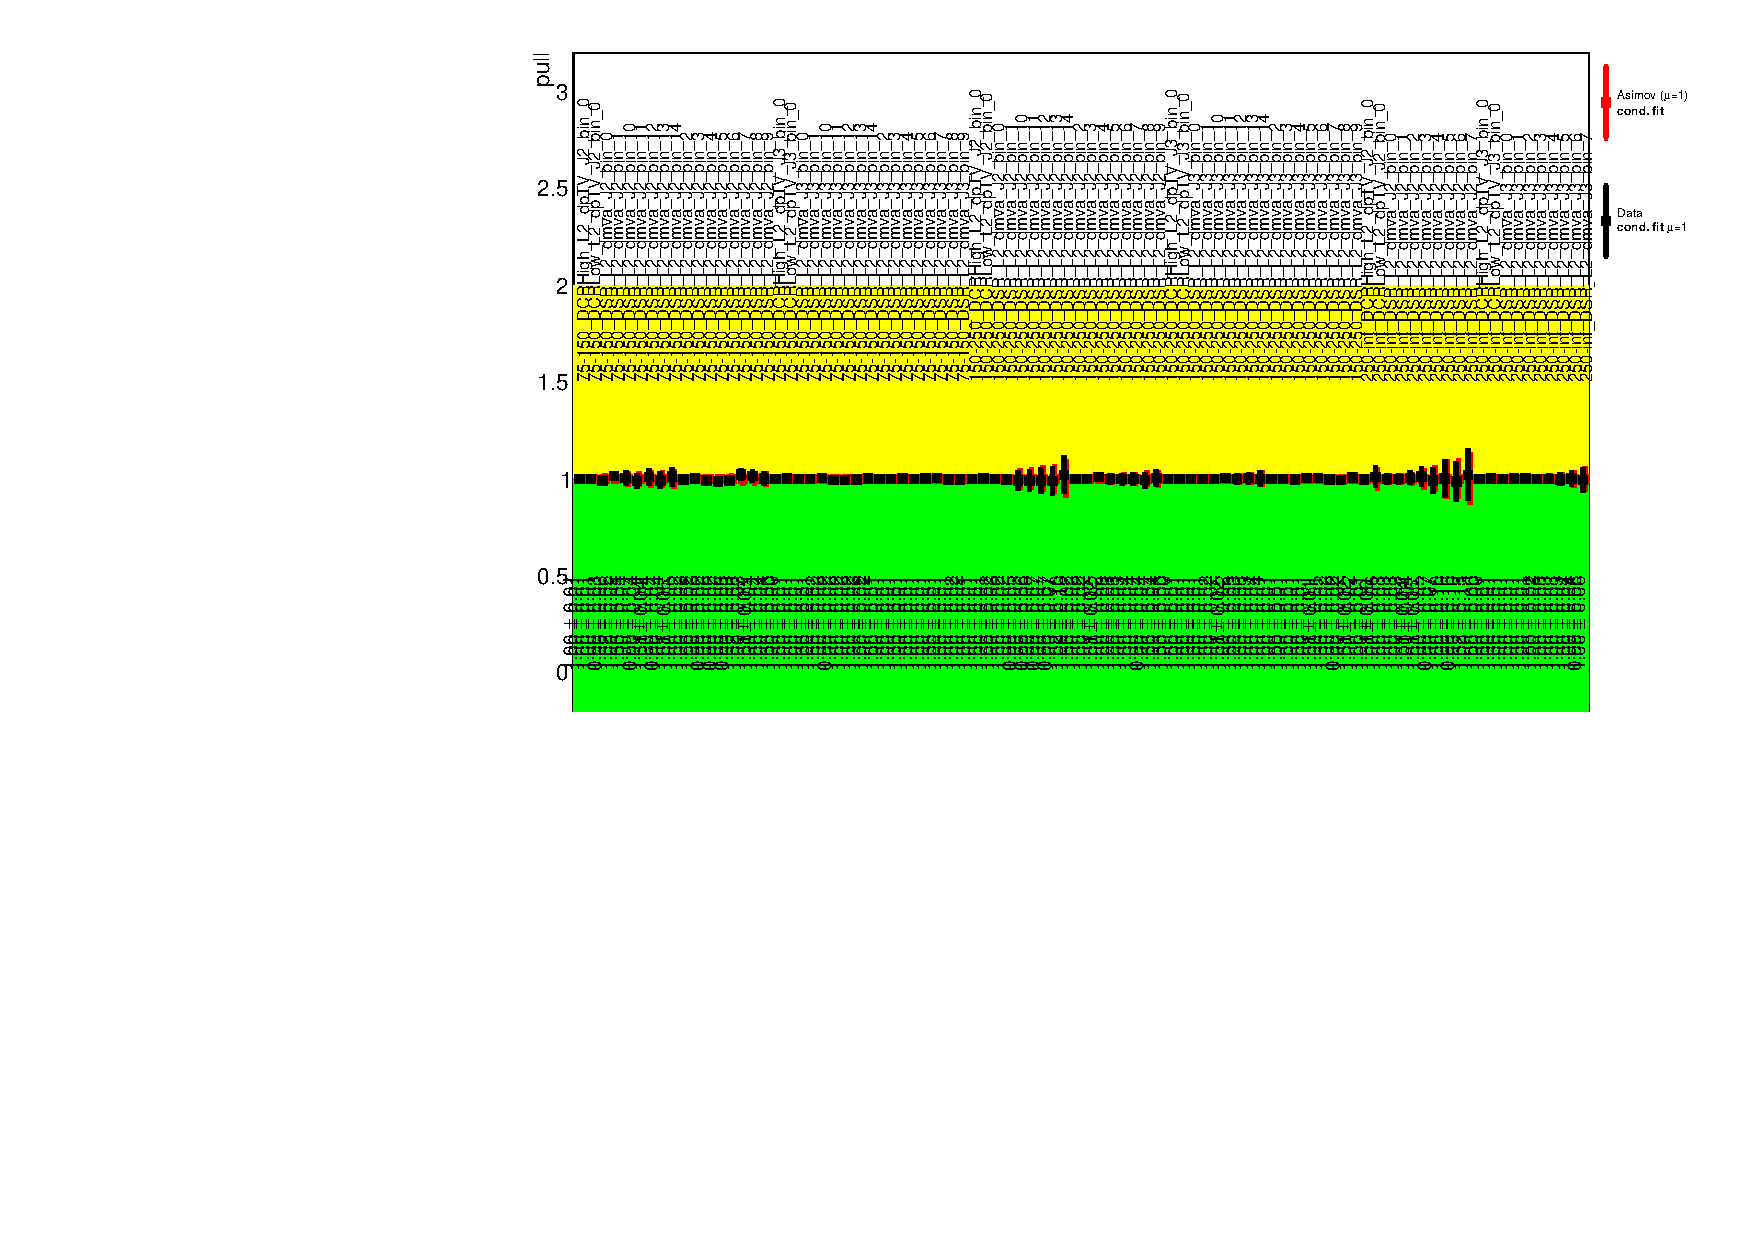
\includegraphics[width=0.49\linewidth]{final_fit_mva/pullComparisons/NP_GammasL2.pdf}
% 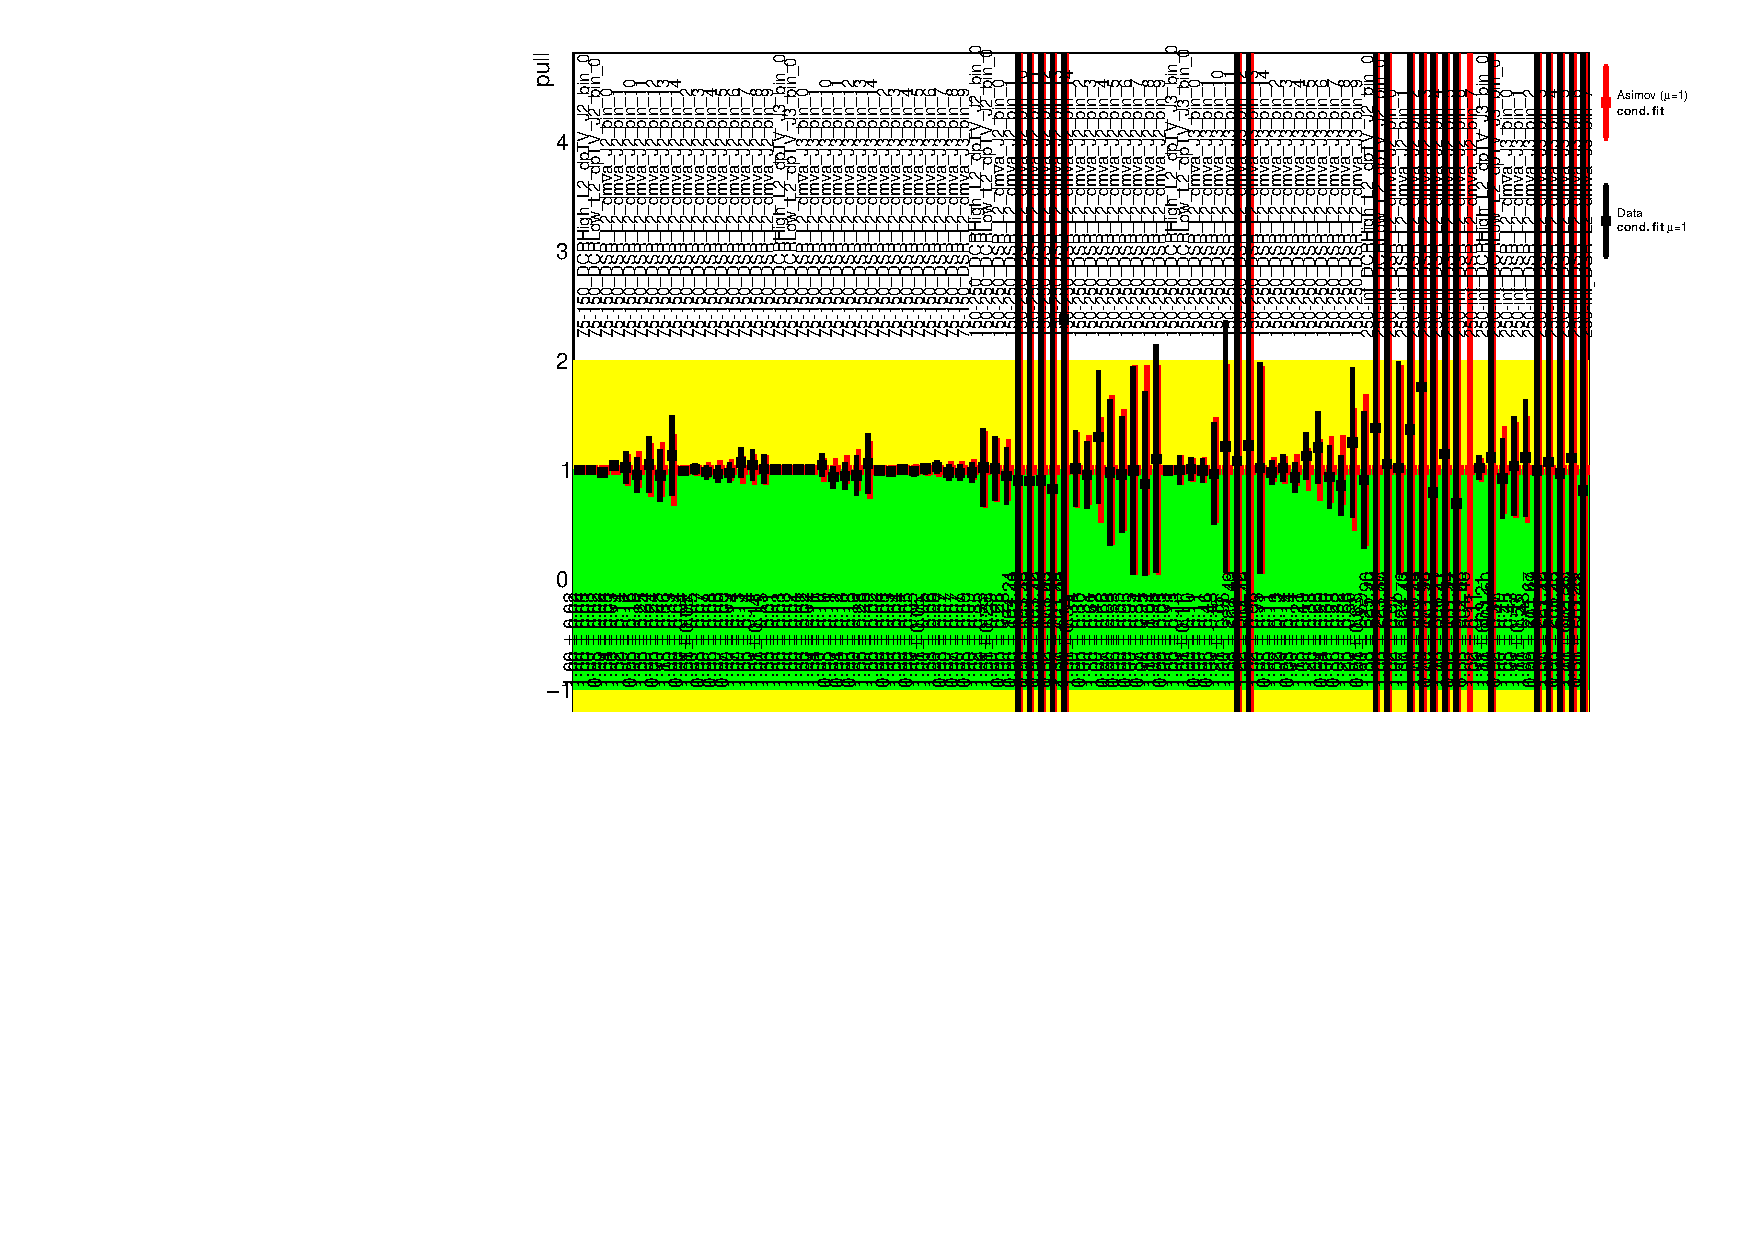
\includegraphics[width=0.49\linewidth]{final_fit_mva/pullComparisons/NP_DDttbar.pdf}
% \caption{caption}
% MC stat. nuisance parameter pulls and the free parameter scale factors
% corresponding to $0$-lepton, $1$-lepton and $2$-lepton as well as the Gamma
% parameter pulls for the data driven top template in the $2$-lepton channel
% corresponding to a conditional combined fit to the Asimov dataset (red) and an
% unconditional combined fit to the \RunTwo data (black)
% \label{fig:nppulls_012L_MVAVH_c} 
% \end{figure}